\documentclass[conference, 10pt,onecolumn]{IEEEtran}
\IEEEoverridecommandlockouts
% The preceding line is only needed to identify funding in the first footnote. If that is unneeded, please comment it out.
\usepackage{cite}
\usepackage{amsmath,amssymb,amsfonts}
\usepackage{algorithmic}
\usepackage{graphicx}
\usepackage{textcomp}
\usepackage{xcolor}
\usepackage{orcidlink}
\usepackage{subcaption}
\usepackage{makecell}
\usepackage[none]{hyphenat}
\usepackage{flushend}

\makeatletter
\newcommand{\linebreakand}{%
\end{@IEEEauthorhalign}
\hfill\mbox{}\par
\mbox{}\hfill\begin{@IEEEauthorhalign}
}
\makeatother
\begin{document}

\title{\textbf{Voice - Based Age and Gender Recognition: A Comparative Study of LSTM, RezoNet and \\ CNN - BiLSTM Hybrid Architecture}\\
}
\author{
\IEEEauthorblockN{1\textsuperscript{st} Nhut Minh Nguyen \orcidlink{0009-0003-1281-5346}}
\IEEEauthorblockA{\textit{Dept. of Artificial Intelligence} \\
\textit{FPT University}\\
Ho Chi Minh City, Vietnam \\
nhutnmse184534@fpt.edu.vn}
\\
\IEEEauthorblockN{3\textsuperscript{rd} Hua Hiep Nguyen \orcidlink{0009-0007-0848-0968}}
\IEEEauthorblockA{\textit{Dept. of Artificial Intelligence} \\
\textit{FPT University}\\
Ho Chi Minh City, Vietnam \\
hiepnhse183787@fpt.edu.vn}
\and
\IEEEauthorblockN{2\textsuperscript{nd} Thanh Trung Nguyen \orcidlink{0009-0004-7553-4848}}
\IEEEauthorblockA{\textit{Dept. of Artificial Intelligence} \\
\textit{FPT University}\\
Ho Chi Minh City, Vietnam \\
trungnt180355@fpt.edu.vn}
\\
\IEEEauthorblockN{4\textsuperscript{th} Dinh Hung Trinh}
\IEEEauthorblockA{\textit{Dept. of Artificial Intelligence} \\
\textit{FPT University}\\
Ho Chi Minh City, Vietnam \\
hungtdse173408@fpt.edu.vn}
}

\maketitle

\begin{abstract}

In this study, the researchers conducted voice-based age and gender recognition using the Common Mozilla Voice dataset in Japanese. This research undertakes a comparative analysis of several deep learning architectures—Long Short-Term Memory networks (LSTMs), Hybrid of Convolutional Neural Networks and Bidirectional Long Short-Term Memory, and the recently introduced RezoNet architecture—for the task of age and gender recognition from voice data. We extracted features such as pitch, magnitude, MFCC, and filter-bank energies from the audio data and compared three architectures: Long - Short Term Memory (LSTM), hybrid of Convolutional Neural Networks and Bidirectional Long Short-Term Memory (CNNs-BiLSTM), and RezoNet architecture. The results revealed that LSTM achieved the highest accuracy for gender recognition 93.5\%, closely followed by CNNs-BiLSTM 93.1\%, with RezoNet performing slightly lower 83.1\%. However, for age recognition, CNNs-BiLSTM outperformed the other models, achieving an accuracy of 69.75\%, while LSTM and RezoNet attained 64.25\% and 44.88\%, respectively. Notably, CNNs-BiLSTM exhibited the highest accuracy across both tasks, underscoring its effectiveness in voice-based age and gender recognition using Japanese language data and the extracted features. These findings suggest promising avenues for future research and applications in this domain.
\end{abstract}

\begin{IEEEkeywords}
Voice Based Age and Gender Recognition, RezoNet, Convolution Neural Network, Long - Short Term Memory (LSTM), Bidirectional Long - Short Term Memory (BiLSTM), Deep Learning.
\end{IEEEkeywords}

\section{Introduction}        
Voice-based recognition systems have become an essential element in various applications, ranging from security systems and customer service automation to personalized user experiences. Among these applications, the ability to accurately determine a speaker's age and gender from voice recordings is particularly valuable for enhancing user interaction and tailoring services more effectively. This study conducts a comparative analysis of various deep learning architectures, including Long Short-Term Memory networks (LSTMs)~\cite{riesmeier2022late}, a hybrid of Convolutional Neural Networks and Bidirectional Long Short-Term Memory (CNNs-BiLSTM)~\cite{kattenborn2021review}, and the newly introduced RezoNet architecture. The objective is to evaluate their performance in age and gender recognition tasks using voice data.

A key aspect of voice-based recognition is understanding waveform differences that correlate with gender and age. Generally, male and female voices exhibit distinct waveform characteristics due to physiological differences in the vocal tract. Male voices typically have lower fundamental frequencies (ranging from 85 to 180 Hz) compared to female voices, is depicted in Figure~\ref{fig:Dataset-Male-Female}, (ranging from 165 to 255 Hz) ~\cite{hanson1999glottal}, resulting in waveforms with longer periods and lower pitch. Age also impacts voice waveforms~\cite{dehqan2013effects}; children's voices have higher pitches and formant frequencies due to their smaller vocal tracts~\cite{lee1999acoustics}, whereas older adults may experience changes in vocal quality and stability due to age-related physiological changes. These variations in pitch, formant frequencies, and vocal tract resonances are crucial for accurately determining age and gender from voice signals~\cite{kent1992acoustic}. To improve these models' performance, extracting meaningful features from the voice recordings is crucial. This study utilizes several feature extraction techniques, including Mel-frequency cepstral coefficients (MFCC)~\cite{1163420}, shifted delta coefficients~\cite{torres2002approaches}, pitch~\cite{yang2016pitch}...


\begin{figure}
    \centering
    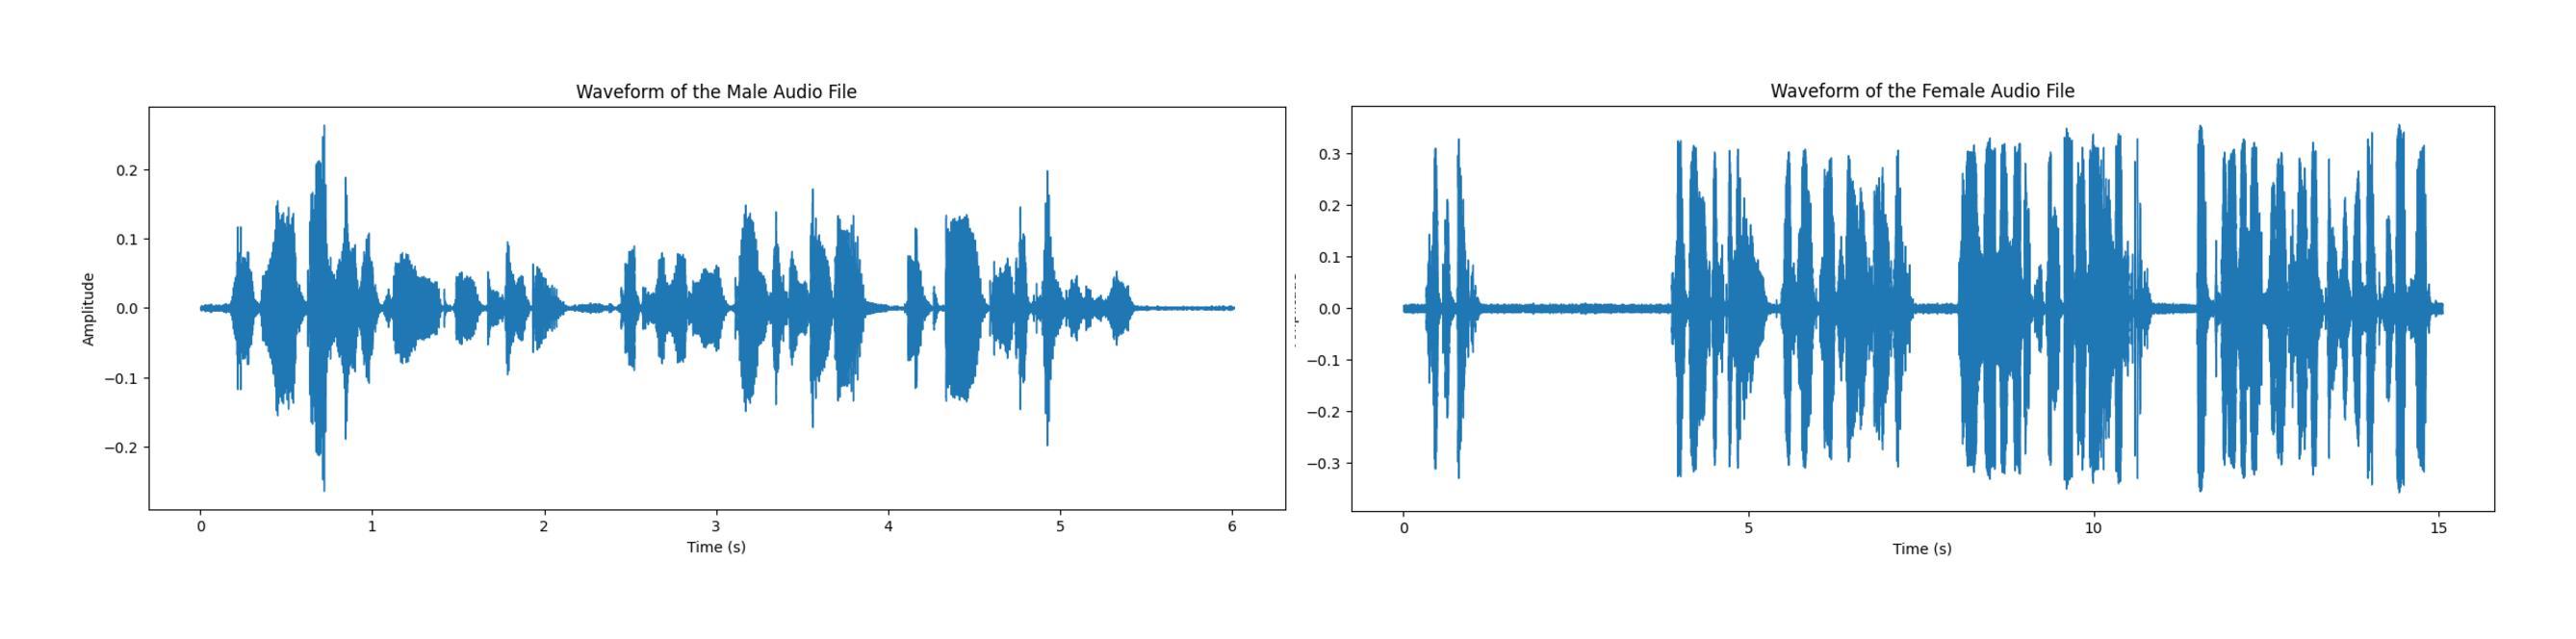
\includegraphics[width=6 in]{Male and Female audio.pdf}
    \caption{Male and Female Audio Signal as Waveform}
    \label{fig:Dataset-Male-Female}
\end{figure}

This study seeks to provide a comprehensive evaluation of these architectures by comparing their performance on a standardized voice dataset. Through the analysis of metrics such as accuracy, precision, recall, and computational efficiency, this research aims to identify the most effective model for real-world applications. Additionally, the study explores the implications of model complexity, training time, and resource requirements, offering insights into the practical deployment of these technologies.

The findings of this research are expected to contribute to the advancement of voice-based recognition systems by providing a detailed understanding of the strengths and limitations of each architecture. This comparative study will serve as a valuable resource for researchers and practitioners aiming to develop more accurate and efficient voice recognition systems tailored to specific demographic characteristics.

The document is organized into several key sections. Section II provides an extensive review of established models and research on the subject, offering valuable insights that help identify areas for improvement, gaps in current knowledge, and alternative strategies. This section also presents evidence supporting the effectiveness of the proposed solution or highlights possible challenges. Section III describes the implemented model, while Section IV outlines the dataset used for both testing and training. Section V summarizes the report's findings and includes a summary of results along with suggestions for future research directions. Section VI is dedicated to acknowledgments, recognizing the contributions and support of individuals and organizations that made this work possible.

\section{Related work}
In this section, we divide our discussion into two parts: one focusing on research employing similar methods, and the other on research utilizing similar technologies.
\subsection{Research Using Similar Methods}
This subsection reviews previous research utilizing similar acoustic and prosodic methods for speaker age and gender identification. Age estimation from speech has garnered increased interest due to its applications in user profiling, targeted marketing, and personalized call routing, which benefit from real-time capabilities. Long short-term memory (LSTM) recurrent neural networks (RNNs) have outperformed state-of-the-art methods in related speech tasks requiring accurate real-time responses. This paper, authored by Ruben Zazo et al~\cite{zazo2018age}, proposes a novel age estimation system based on LSTM-RNNs that handles short utterances (3 to 10 seconds) and can be deployed in real-time architectures. Tested against a state-of-the-art i-vector approach using NIST speaker recognition evaluation 2008 and 2010 data sets, the proposed system shows up to a 28\% relative improvement in mean absolute error for short-duration utterances.

Abhishek Singhal and Devendra Kumar Sharma~\cite{abdi2010principal} explore gender identification from voice signals across different age groups using various classification algorithms. The paper evaluates recall values for genders within teenage, middle, and old age groups, employing Mel Frequency Cepstral Coefficients (MFCCs) as extracted features. Linear Discriminant Analysis (LDA), Recurrent Neural Network Bidirectional Long Short-Term Memory (RNN-BiLSTM), and Support Vector Machine (SVM) algorithms are utilized for classification. Results indicate that RNN exhibits the highest recall values for both male and female genders across different age groups, outperforming SVM and LDA. Specifically, RNN achieves the highest recall values for males in the teenage group and for females in the old age group, surpassing other algorithms in accuracy.

Yong Yu, Xiaosheng Si, Changhua Hu, and Jianxun Zhang~\cite{yu2019review} explore the advancements and applications of long short-term memory (LSTM) in the field of recurrent neural networks (RNNs). While traditional RNNs with sigma or tanh cells struggle with learning relevant information when there are large gaps in the input data, LSTMs address this issue effectively through gate functions that manage long-term dependencies. Since their introduction, LSTMs have achieved significant results and have become central to deep learning research. The paper reviews LSTM cells and their variants, categorizing LSTM networks into LSTM-dominated and integrated LSTM networks, and discusses their diverse applications. Future research directions for LSTM networks are also presented.

Vinayak Sudhakar Kone et al.~\cite{kone2023voice} explore a machine learning-based approach for gender and age detection using voice data. We investigate various feature extraction techniques and evaluate different machine-learning algorithms for classification. We discuss this research area's potential benefits and challenges and highlight open issues for future exploration. Their proposed method utilizes a grid search pipeline with RobustScaler~\cite{qian2022robustscaler}, Principal Component Analysis (PCA)~\cite{abdi2010principal}, and Logistic Regression~\cite{lavalley2008logistic} for age prediction. For gender classification, we employ a sequential model with five hidden layers. This approach achieved an accuracy of 91\% for gender and 59\% for age on the Common Voice dataset.

Ming Li et al. \cite{li2013automatic} presents a novel approach to automatic speaker age and gender identification by combining seven methods at acoustic and prosodic levels to improve baseline performance. The baseline subsystems include Gaussian mixture model (GMM) with mel-frequency cepstral coefficients, support vector machine (SVM) with GMM mean supervectors, and an SVM with 450-dimensional utterance-level features. Four new subsystems are introduced, involving SVMs and sparse representations using various supervectors and prosodic features. These new subsystems effectively classify age and gender groups, and their weighted fusion enhances overall performance. Tested on the 2010 Interspeech Paralinguistic Challenge~\cite{velichko2022complex} a Gender database, the fusion system improves unweighted accuracy by 5.6\% for age and 4.2\% for gender on the development set, and by 3.1\% and 3.8\% respectively on the final test set, compared to the baseline.

\subsection{Research Using Similar Technology}
While the previous section focused on voice-based age and gender detection, this subsection will explore the application of similar voice analysis technologies in distinct areas. Sera Kim and Seok-Pil Lee present a study focusing on advancing emotion recognition from speech using dimensionality reduction algorithms for visualization to highlight emotion-specific audio features \cite{kim2023bilstm}. The proposed model architecture combines bidirectional long short-term memory (BiLSTM)–Transformer and a 2D convolutional neural network (CNN). The BiLSTM–Transformer captures speech pattern sequences, while the 2D CNN handles Mel-Spectrograms for spatial audio details. Validated using 10-fold cross-validation, the model achieves high unweighted accuracy rates of 95.65\% and 80.19\% on Emo-DB and RAVDESS databases, respectively. These findings suggest that the proposed transformer-based deep learning model, coupled with appropriate feature selection, significantly enhances emotion recognition from speech.

Li-Min Zhang and colleagues explore how gender differences in speech affect emotion recognition~\cite{zhang2023deep} accuracy, proposing a method to improve it by using gender-specific features. The study begins with classifying speech by gender using a Multi-Layer Perceptron (MLP). It then analyzes the impact of various acoustic features on emotion recognition for male and female speech, establishing optimal feature sets for each gender. These sets are used to train and test Convolutional Neural Networks (CNN) and Bidirectional Long Short-Term Memory networks (BiLSTM). The results demonstrate that the proposed gender-specific emotion recognition models outperform gender-mixed models in terms of average recognition accuracy.

Sidra Abid Syed discusses the role of computerized acoustic examination in early diagnosis and monitoring of pathological speech~\cite{syed2021comparative}. The study aims to detect diseases from voice using various acoustic metrics, which are influenced by speech noise detection algorithms. The methodology involves feature extraction from the SVD dataset, followed by input into a 27-layer neural network comprising convolutional and recurrent layers. The dataset is divided for training and testing, and 10-fold cross-validation is employed to assess performance. The reported accuracies are 87.11\% for CNN and 86.52\% for RNN. The program, written in Python using TensorFlow, was executed on a Linux workstation with an NVidia Titan X GPU.

\section{Proposed Method}

This section delves into a method we explored for recognizing age and gender based on voice data. We assessed the performance of three distinct architectures: Long - Short Term Memory (LSTM)\cite{riesmeier2022late}, RezoNet Architecture, and a hybrid of Convolutional Neural Networks Bidirectional Long Short-Term Memory Architecture (CNN-BiLSTM)~\cite{kattenborn2021review}. The system functions in two primary stages: training and testing, in Figure~\ref{fig:Research Architecture}. During the training stage, audio data is input into the system, where it undergoes several processing steps including voice activity detection to isolate speech from noise, feature extraction to obtain features like MFCCs~\cite{1163420}, pitch\cite{yang2016pitch}, magnitude\cite{torres2002approaches}, and filter bank energies, and normalization to ensure consistency. In the testing stage, new audio data is processed similarly, and the extracted features are fed into separate models for gender and age recognition. These models, employing LSTM, RezoNet, or hybrid CNN-BiLSTM architectures, analyze the features to predict the speaker's gender and age. Essentially, we compared these three model architectures to determine the most effective for voice-based age and gender recognition.

\begin{figure}
    \centering
    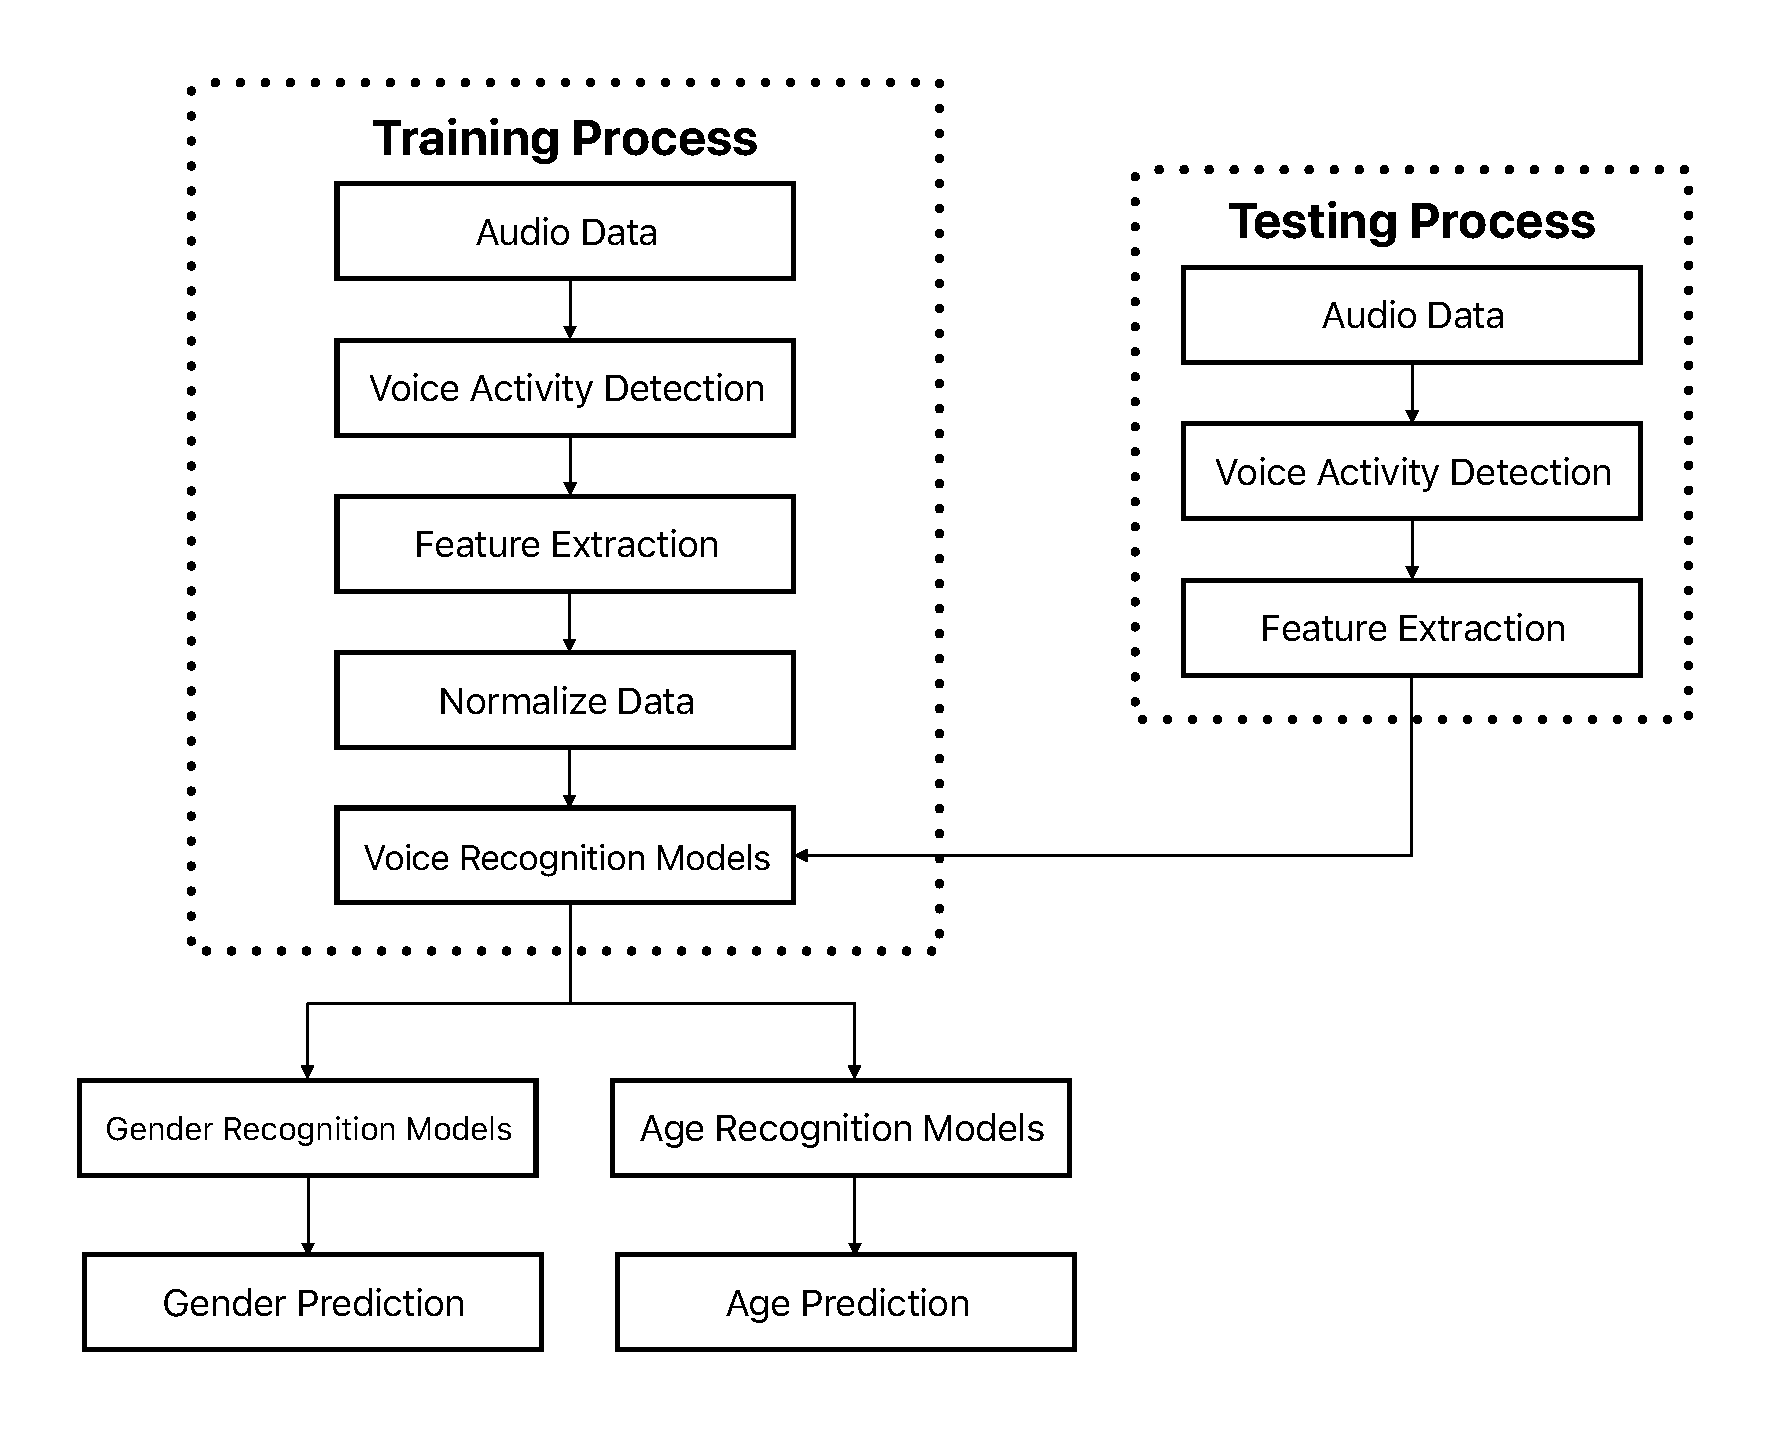
\includegraphics[width=3.5 in]{Research Architecture.pdf}
    \caption{Architecture of Voice-based Age and Gender Recognize System}
    \label{fig:Research Architecture}
\end{figure}

\subsection{Long - Short Term Memory Architecture}
Voice-based age and gender classification involves analyzing audio signals to predict a speaker's age and gender. Long Short-Term Memory (LSTM) networks~\cite{yu2019review}, the LSTM architecture of our research is visualized in Figure~\ref{fig:LSTM architecture}, a type of recurrent neural network (RNN), are well-suited for this task due to their ability to capture temporal dependencies in sequential data, such as audio signals.

\begin{figure}
    \centering
    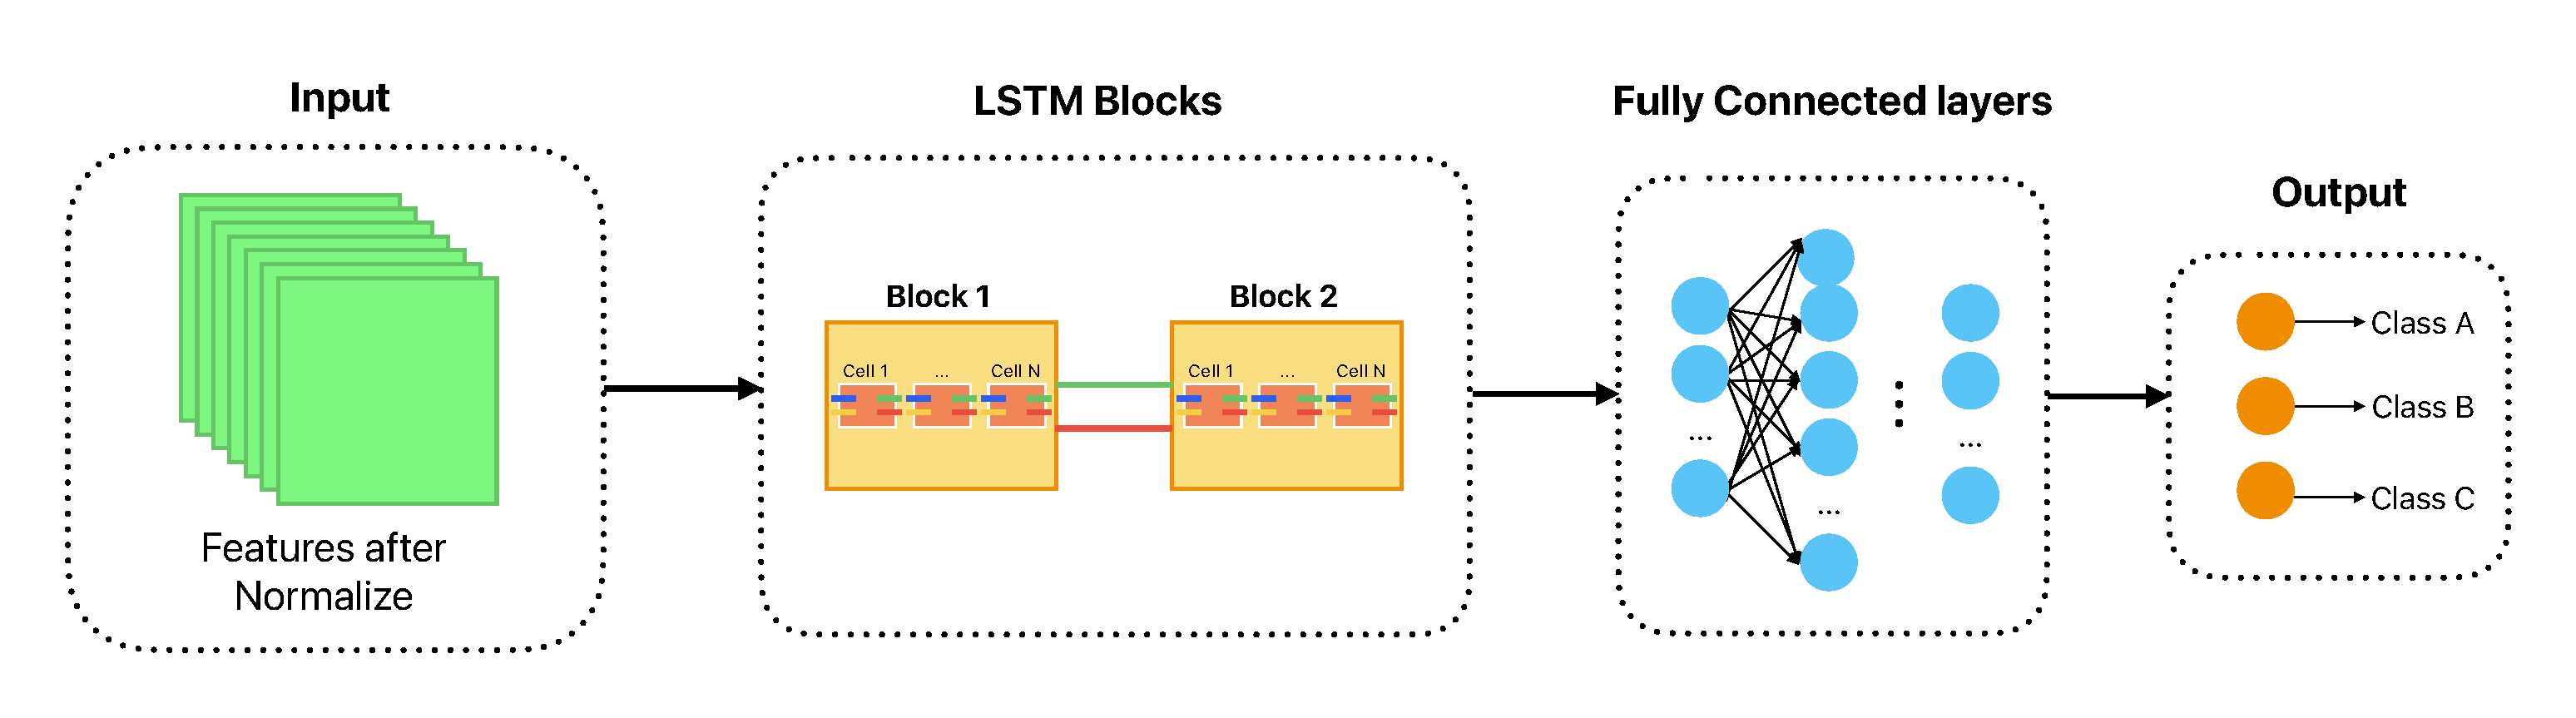
\includegraphics[width=6 in]{LSTM architecture.pdf}
    \caption{LSTM Architecture}
    \label{fig:LSTM architecture}
\end{figure}

LSTM networks are constructed from LSTM cells~\cite{yu2019review}, which defined by the following Figure~\ref{fig:LSTM cell architecture}, which are designed to mitigate the vanishing gradient problem prevalent in traditional RNNs. Each LSTM cell consists of several crucial components~\cite{smagulova2019survey}:
\begin{itemize}
    \item Cell State (\(C_t\)): This serves as the cell's memory, preserving information across time steps. The candidate Cell State~\ref{eq:candidate_cell_state} and updated Cell State~\ref{eq:update_cell_state} are defined by the following equations.
    % Candidate Cell State
    \begin{equation}
        \tilde{C}_t = \tanh(W_C [h_{t-1}, x_t] + b_C)
        \label{eq:candidate_cell_state}
    \end{equation}
    % Update Cell State
    \begin{equation}
        C_t = f_t \ast C_{t-1} + i_t \ast \tilde{C}_t
        \label{eq:update_cell_state}
    \end{equation}
        Where: \(W\) represents the weight matrices, $\tanh$ represents the hyperbolic tangent function.
    \item Hidden State (\(h_t\)): This represents what the cell outputs, capturing relevant information from the current audio and what it "remembered" before. There's another equation~\ref{eq:hidden_state} for this.
    % Hidden State
    \begin{equation}
        h_t = o_t \ast \tanh(C_t)
        \label{eq:hidden_state}
    \end{equation}
        Where: \(\sigma\) represents the sigmoid function, $\tanh$ represents the hyperbolic tangent function.
    \item Input Gate (\(i_t\)): This gate controls how much new information gets added to the memory cell. An equation~\ref{eq:input_gate} defines its function.
    % Input Gate
    \begin{equation}
        i_t = \sigma(W_i [h_{t-1}, x_t] + b_i)
        \label{eq:input_gate}
    \end{equation}
        Where: \(W\) represents the weight matrices, \(\sigma\) represents the sigmoid function, \(b_i\) represents the bias vector for the input gate.
    \item Forget Gate (\(f_t\)): This gate decides how much of the past information to keep in the memory. There's an equation~\ref{eq:forget_gate} for this as well.
    % Forget Gate
    \begin{equation}
        f_t = \sigma(W_f [h_{t-1}, x_t] + b_f)
        \label{eq:forget_gate}
    \end{equation}
        Where: \(W\) represents the weight matrices, \(\sigma\) represents the sigmoid function, \(b_f\) represents the bias vector for the forget gate.
    \item Output Gate (\(o_t\)): This gate determines how much information from the memory cell is sent on to the next processing stage. Yet another equation~\ref{eq:output_gate} defines this gate's role.
    % Output Gate
    \begin{equation}
        o_t = \sigma(W_o [h_{t-1}, x_t] + b_o)
        \label{eq:output_gate}
    \end{equation}
        Where: \(W\) represents the weight matrices, \(\sigma\) represents the sigmoid function, \(b_o\) represents the bias vector for the output gate.
\end{itemize}

\begin{figure}
    \centering
    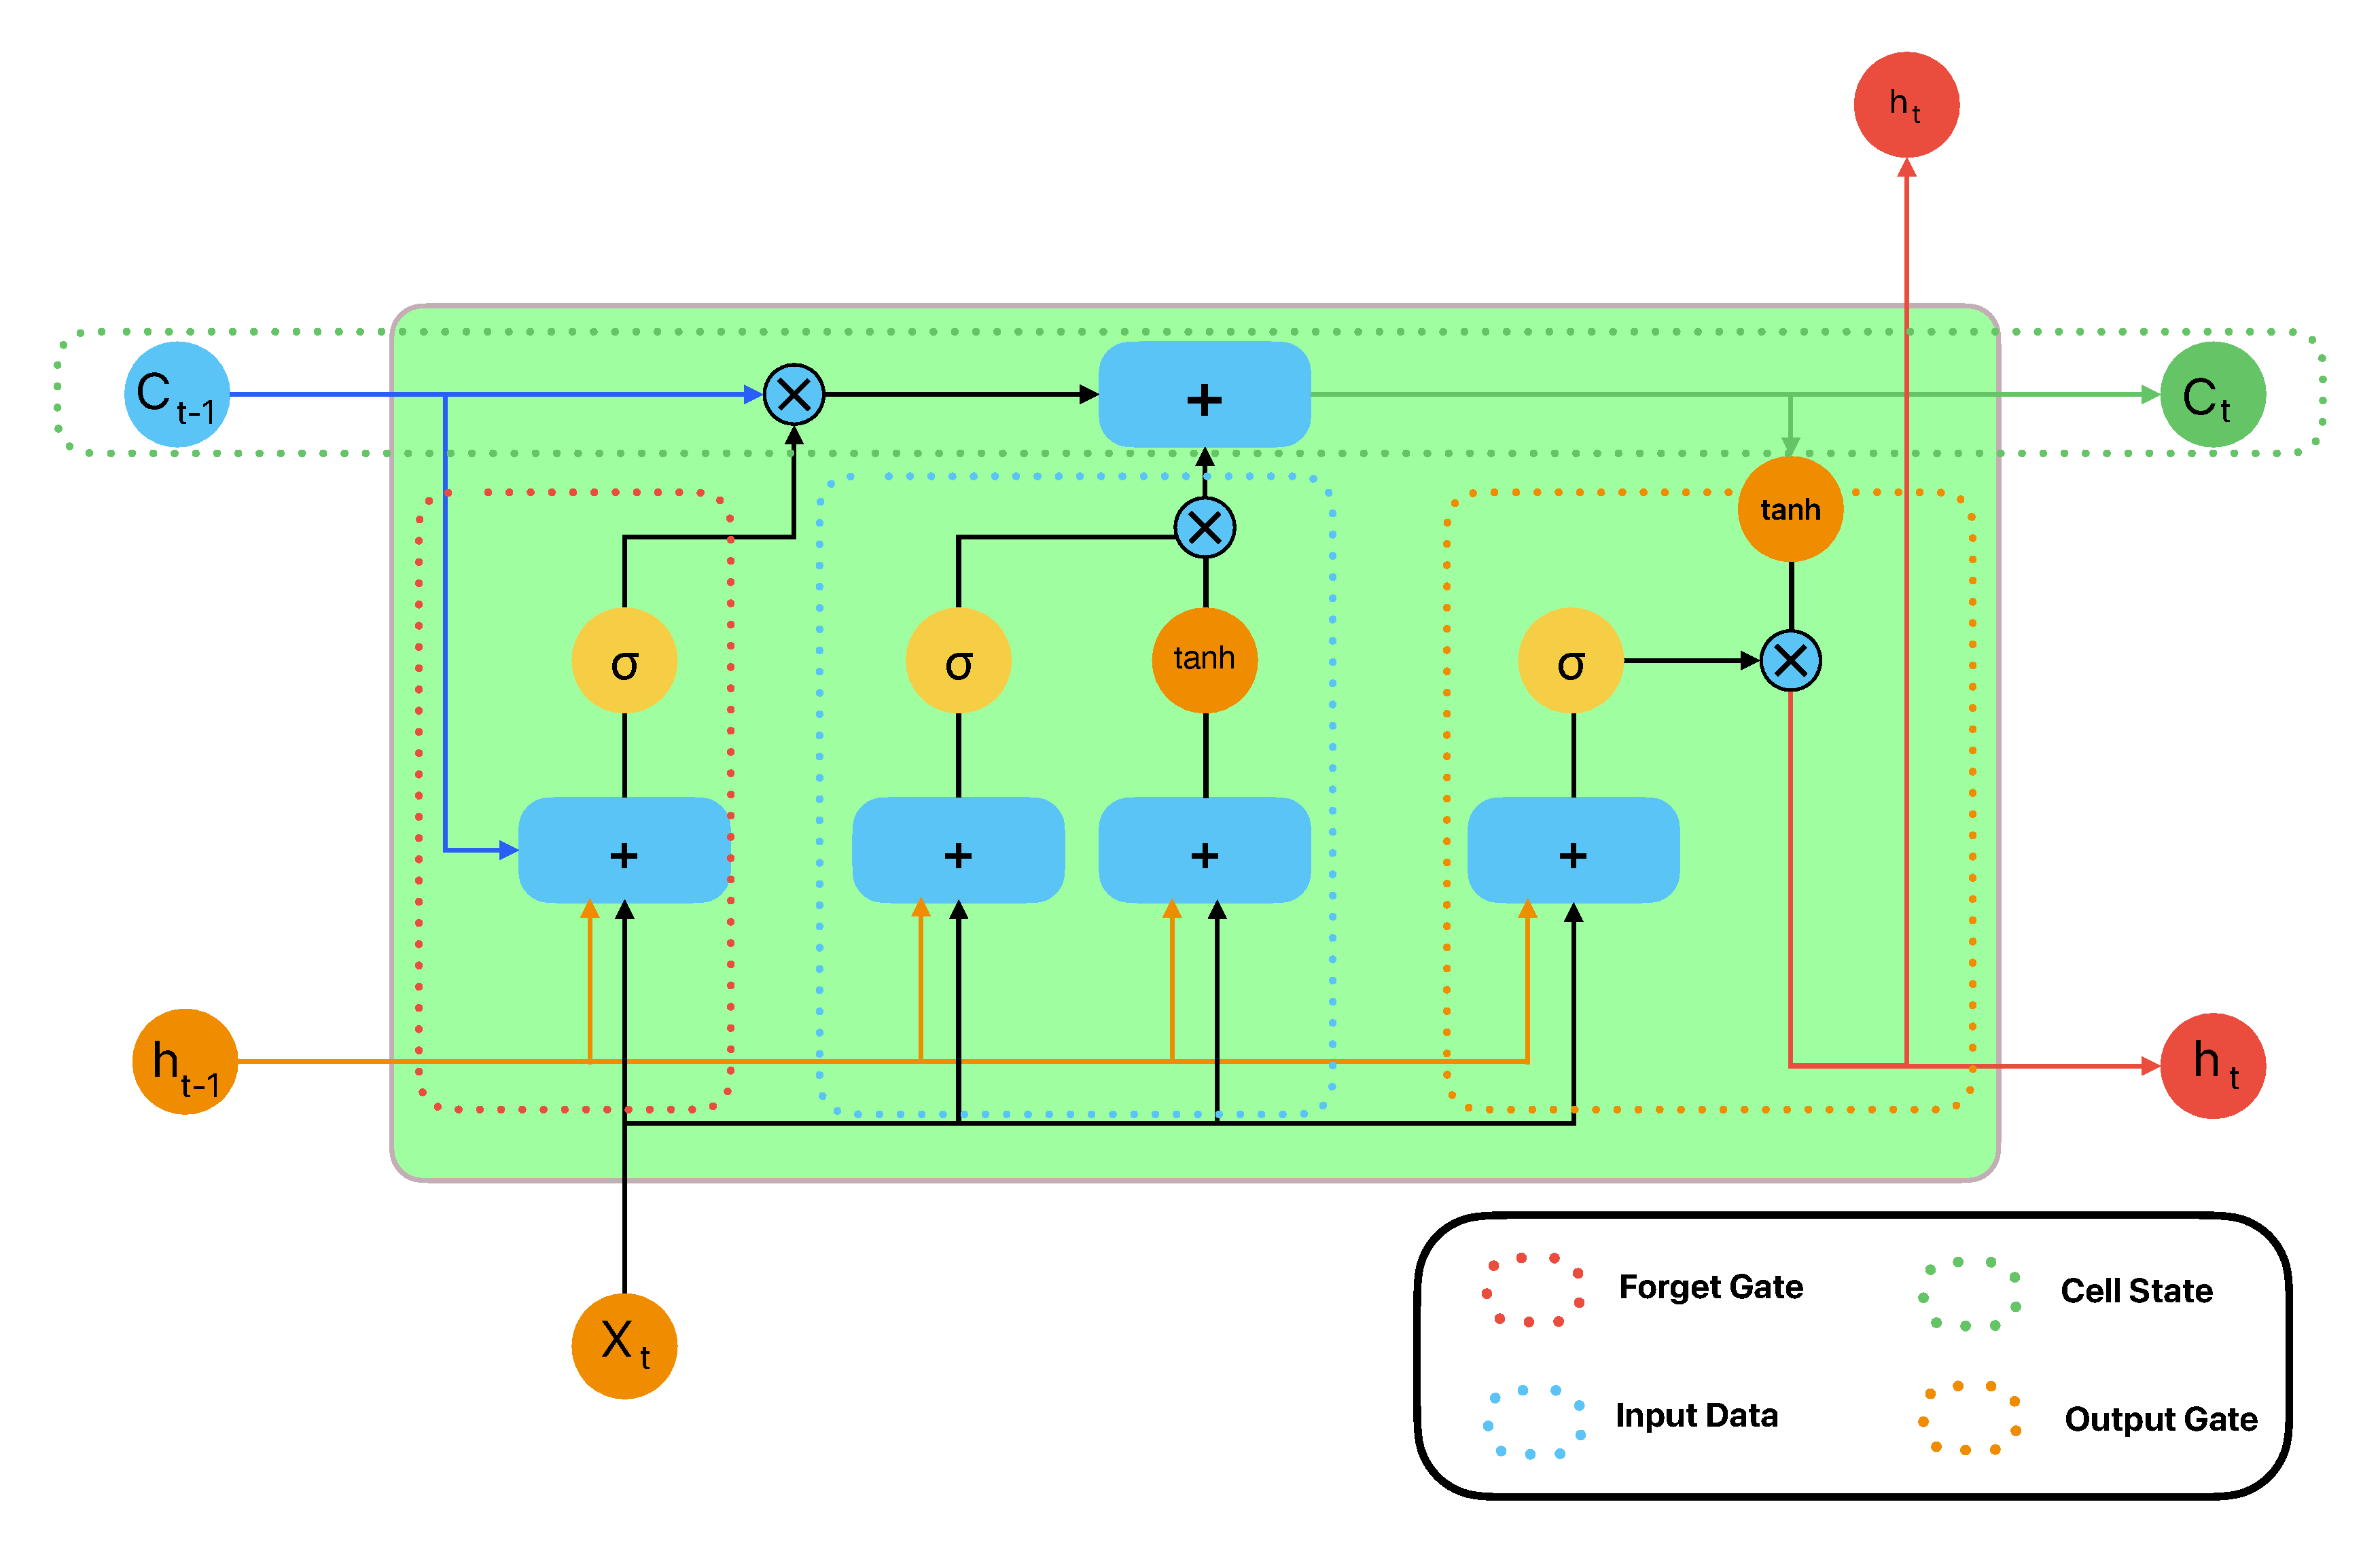
\includegraphics[width=3.5 in]{LSTM cell architecture.pdf}
    \caption{LSTM Cell architecture}
    \label{fig:LSTM cell architecture}
\end{figure}

For the gender prediction model, as depicted in Table \ref{tab:LSTM_Gender}, the input layer takes data with a shape of (128, 35, 54), with the batch size is 128, 35 signifies the sequence length, and 54 denotes the feature dimension. This data is then fed into an LSTM layer with 256 nodes, resulting in an output shape of (128, 35, 256). Subsequently, another LSTM layer with 128 nodes, incorporating dropout of 0.3 and batch normalization, processes the data to yield an output shape of (128, 256). Following this, there are three dense layers, each preceded by dropout of 0.3 and batch normalization. The first dense layer has 256 nodes, the second has 128 nodes, and the third has 64 nodes. Finally, the output layer comprises 5 nodes, representing the different gender classes, with an output shape of (128, 5).

On the other hand, the LSTM age model, detailed in Table \ref{tab:LSTM_Age}, it shares a similar initial structure with the gender model, with an input layer accepting data of shape (128, 35, 54). However, the subsequent LSTM layer differs slightly, as it outputs data with shape (128, 35, 256), suggesting a possible oversight in the table with an additional comma. The following LSTM layer with 128 nodes, dropout, and batch normalization processes the data to produce an output shape of (128, 256). The subsequent dense layers again incorporate dropout and batch normalization, with the first dense layer having 256 nodes and the second dense layer having 128 nodes. Notably, the third dense layer has 128 nodes, which might be an inadvertent inconsistency in the table. Finally, similar to the gender model, the output layer consists of 5 nodes, representing different age classes, with an output shape of (128, 5).

These architectures leverage LSTM layers to capture temporal dependencies in the voice data, while the subsequent dense layers help in feature extraction and classification. The inclusion of dropout and batch normalization aids in regularization and stabilizes the training process, contributing to the model's robustness and generalization ability.

\begin{table}[]
    \centering
    \begin{tabular}{|c|c|c|}
        \hline
        \textbf{Layer} & \textbf{Nodes} & \textbf{Output Shape} \\ \hline
        \textbf{Input Layer} & & (128, 35, 54)\\
        \textbf{LSTM} & 256 & (128, 35, 256)\\
        \textbf{LSTM} (Dropout (0.3), BatchNormalization) & 128 & (128, 256)\\
        \textbf{Dense} (Dropout (0.3), BatchNormalization) & 256 & (128, 256)\\
        \textbf{Dense} (Dropout (0.3), BatchNormalization) & 128 & (128, 128)\\
        \textbf{Dense} (Dropout (0.3), BatchNormalization) & 64 & (128, 64)\\
        \textbf{Output Layer} & 5 & (128, 5)\\
         \hline
    \end{tabular}
    \caption{The parameters of LSTM Gender Model}
    \label{tab:LSTM_Gender}
\end{table}

\begin{table}[]
    \centering
    \begin{tabular}{|c|c|c|}
    \hline
        \textbf{Layer} & \textbf{Nodes} & \textbf{Output Shape} \\ \hline
        \textbf{Input Layer} & & (128, 35, 54)\\
        \textbf{LSTM} & 256 & (128, ,35, 256)\\
        \textbf{LSTM} (Dropout (0.3), BatchNormalization) & 128 & (128, 256)\\
        \textbf{Dense} (Dropout (0.3), BatchNormalization) & 256 & (128, 256)\\
        \textbf{Dense} (Dropout (0.3), BatchNormalization) & 128 & (128, 128)\\
        \textbf{Dense} (Dropout (0.3), BatchNormalization) & 128 & (128, 128)\\
        \textbf{Dense} (Dropout (0.3), BatchNormalization) & 64 & (128, 64)\\
        \textbf{Output Layer} & 5 & (128, 5)\\
        \hline
    \end{tabular}
    \caption{The parameters of LSTM Age Model}
    \label{tab:LSTM_Age}
\end{table}

\subsection{RezoNet Architecture}

This subsection provides a detailed description of the RezoNet architecture, as depicted in Figure~\ref{fig:RezoNet Architecture}, which is specifically tailored for identifying age and gender from voice data. It utilizes a combination of convolutional and residual blocks, along with dense layers, to extract features and make accurate predictions. 

The RezoNet architecture initiates with an input layer processing audio data, incorporating an initial Conv2D layer with batch normalization, max pooling, and dropout for initial feature extraction. Subsequently, a sequence of residual blocks follows, each consisting of Conv2D layers, batch normalization, max pooling, and dropout, along with shortcut connections to aid in gradient flow. After these blocks, a Flatten layer reshapes the data into a 2D form, which then proceeds to fully connected dense layers, each incorporating dropout and batch normalization for regularization and stability. Ultimately, the output layer produces predictions for age and gender categories.

The residual block~\cite{park2022generative} design within RezoNet, illustrated in Figure~\ref{Residual Block Architecture}, introduces shortcut connections to address training challenges in deep neural networks. These connections alleviate issues such as vanishing gradients by facilitating smoother gradient flow and enabling the training of deeper networks. This approach enhances performance and convergence by effectively retaining and leveraging information from earlier layers. Each residual block comprises Conv2D layers for feature extraction, followed by batch normalization for stabilizing the learning process. MaxPooling2D layers downsample feature maps, while dropout prevents overfitting. A key aspect of the residual block is the shortcut connection, which directly adds the input of the block to its output, facilitating gradient flow through the network and addressing the vanishing gradient problem.

In the RezoNet architecture, Conv2D~\cite{agarwal2021new} plays a crucial role in feature extraction for voice-based age and gender classification. Conv2D, a fundamental component of convolutional neural networks (CNNs), convolves learnable filters over input spectrogram data, capturing intricate patterns indicative of age and gender characteristics in voice recordings. By employing Conv2D layers, RezoNet effectively extracts discriminative features from spectrograms, enabling subsequent layers to learn hierarchical representations crucial for accurate age and gender classification. Leveraging Conv2D within the RezoNet architecture enables the model to discern subtle variations in vocal features, contributing to robust and precise predictions of age and gender from audio inputs.

The RezoNet Gender Model, depicted in Table~\ref{tab:RezoNet_Gender}, is designed for gender recognition based on voice data. It begins with an input layer processing audio data of shape (128, 35, 54, 1). The subsequent layers consist of Conv2D with batch normalization, max pooling, and dropout, followed by several residual blocks. These residual blocks progressively downsample the data and increase the depth of features extracted. After the residual blocks, the data is flattened into a shape of (128, 512) and fed into dense layers with dropout and batch normalization for regularization. Finally, the output layer produces predictions for two gender categories.

In contrast, the RezoNet Age Model, outlined in Table~\ref{tab:RezoNet_Age}, is tailored for age recognition from voice data. It shares the same initial layers as the gender model but differs in the number of nodes in the Conv2D layers and the structure of residual blocks. These variations accommodate the complexity of age prediction, with deeper residual blocks and larger Conv2D layers to capture more intricate age-related features. The flattened data is reshaped to (128, 3072) before passing through dense layers and finally predicting age categories using the output layer with five nodes.

In summary, the RezoNet architecture, designed for age and gender identification from voice data, employs convolutional and residual blocks alongside dense layers for accurate predictions. It begins with an initial Conv2D layer for feature extraction, followed by residual blocks with shortcut connections to facilitate gradient flow. Conv2D layers play a crucial role in capturing intricate patterns in voice recordings, enabling the model to discern subtle variations important for classification. The Gender Model predicts gender categories, while the Age Model, with deeper residual blocks and larger Conv2D layers, specializes in age prediction.

\begin{figure}
    \centering
    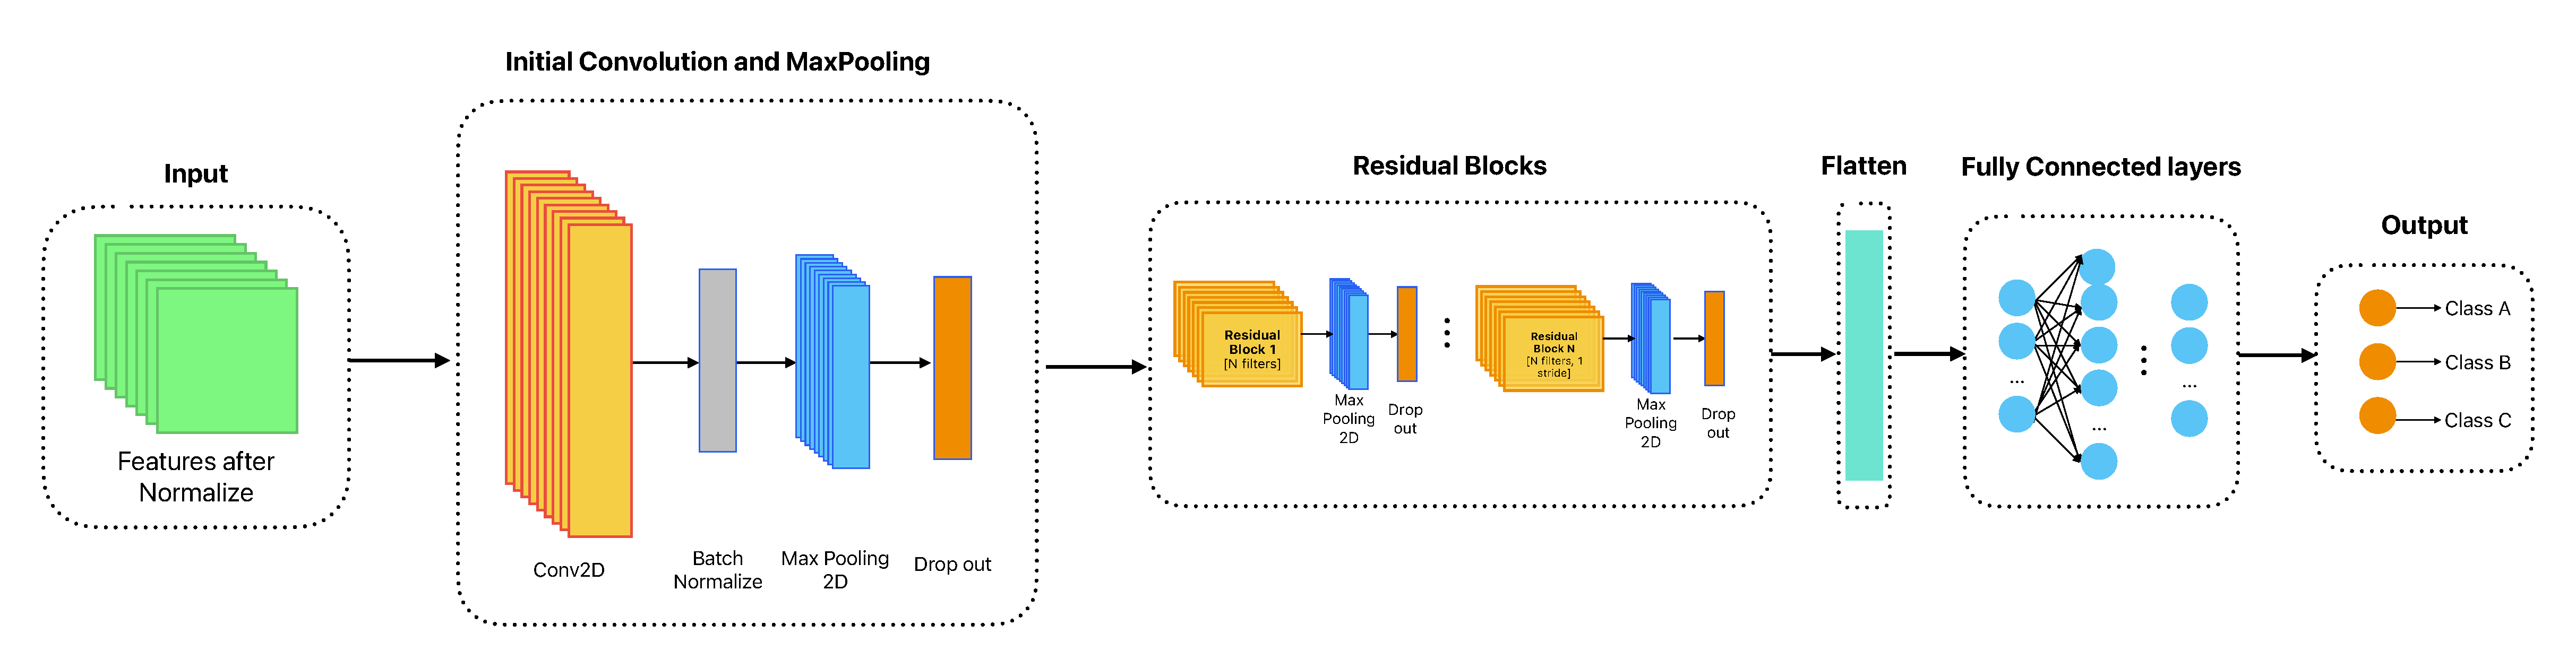
\includegraphics[width=7 in]{RezoNet Architecture.pdf}
    \caption{RezoNet Architecture}
    \label{fig:RezoNet Architecture}
\end{figure}

\begin{figure}
    \centering
    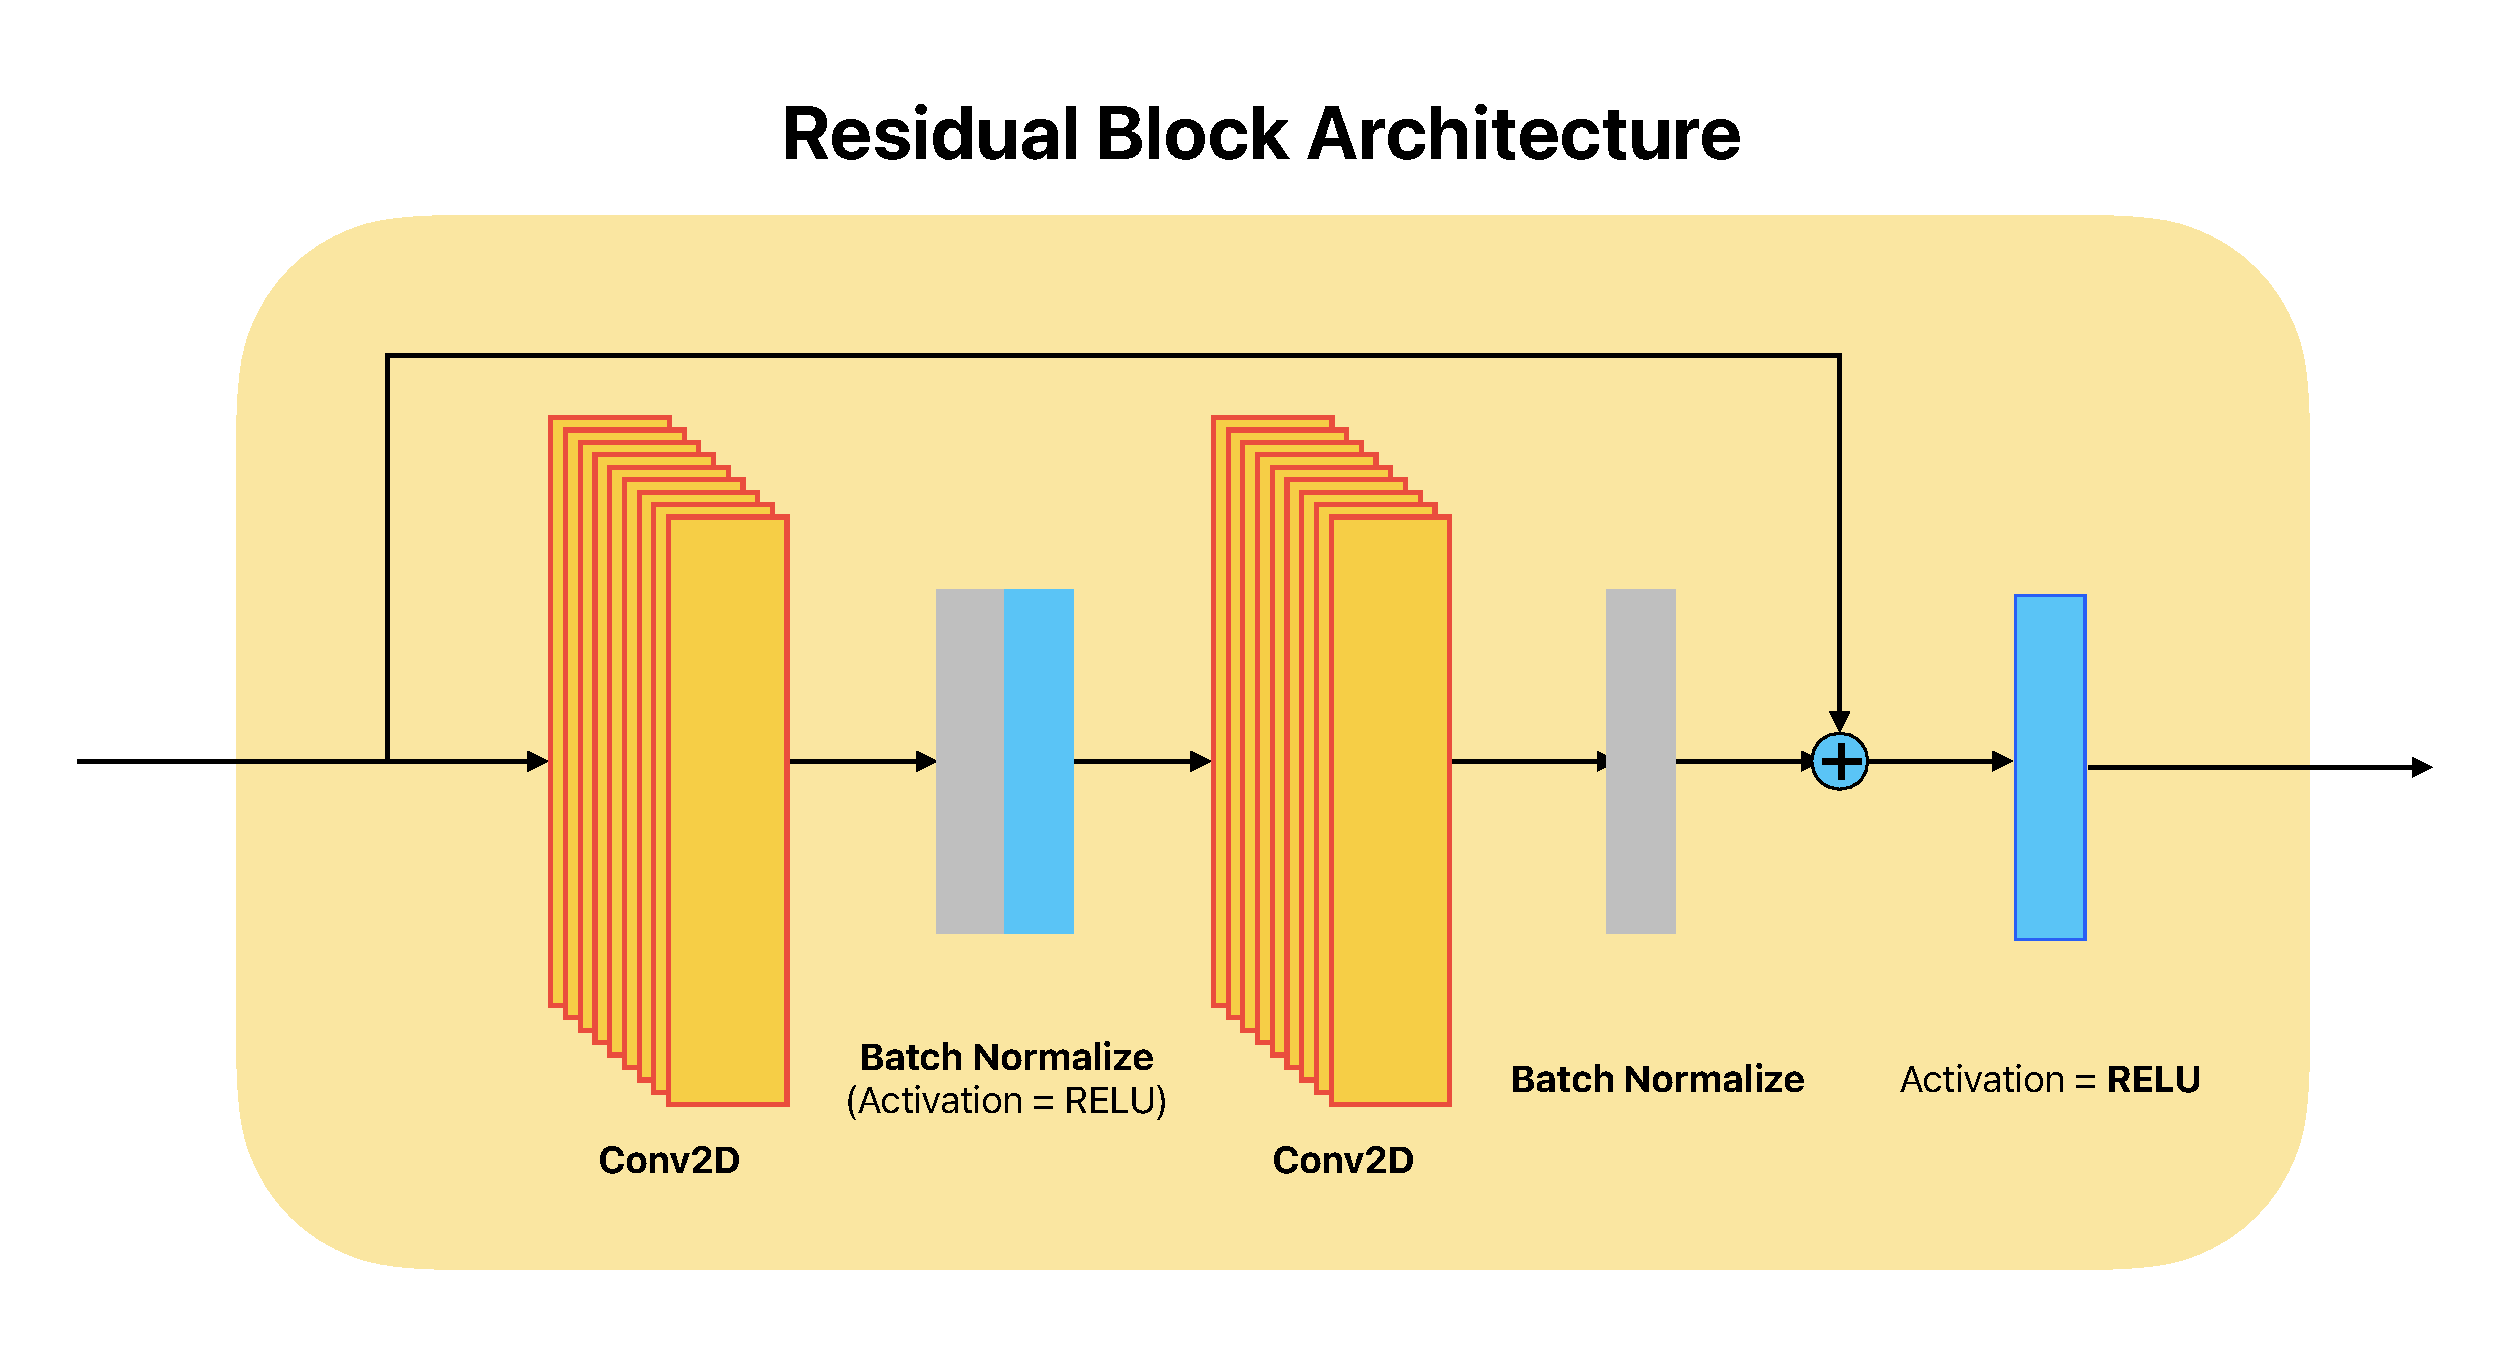
\includegraphics[width=3 in]{Residual Block Architecture.pdf}
    \caption{Residual Block Architecture}
    \label{Residual Block Architecture}
\end{figure}

\begin{table}[]
    \centering
    \begin{tabular}{|c|c|c|}
        \hline
        \textbf{Layer} & \textbf{Nodes} & \textbf{Output Shape} \\ \hline
        \textbf{Input Layer} & & (128, 35, 54, 1)\\
        \textbf{Conv2D} (BatchNormalization, MaxPooling2D, Dropout (0.3)) & 32 & (128, 17, 27, 32)\\
        \textbf{Residual blocks} (MaxPooling2D (Pool Size=(2, 2)), Dropout(0.3))& 32& (128, 8, 13, 64)\\
        \textbf{Residual blocks} (MaxPooling2D (Pool Size=(2, 2)), Dropout(0.3))& 64&  (128, 4, 6, 64)  \\
        \textbf{Residual blocks} (MaxPooling2D (Pool Size=(2, 2), Dropout(0.3))& 128&  (128, 2, 3, 128)\\
        \textbf{Residual blocks} (MaxPooling2D (Pool Size=(1, 2)), Dropout (0.3))& 256& (128, 2, 1, 256)\\
        \textbf{Flatten} & & (128, 512) \\
        \textbf{Dense} (Dropout (0.3), BatchNormalization) & 128&  (128, 128)\\
        \textbf{Dense} (Dropout (0.3), BatchNormalization) & 64 & (128, 64)\\       
        Output & 2 & (128, 2)\\
         \hline
    \end{tabular}
    \caption{The parameters of RezoNet Architecture Gender Model}
    \label{tab:RezoNet_Gender}
\end{table}

\begin{table}[]
    \centering
    \begin{tabular}{|c|c|c|}
        \hline
        \textbf{Layer} & \textbf{Nodes} & \textbf{Output Shape} \\ \hline
        \textbf{Input Layer} & & (128, 35, 54, 1)\\
        \textbf{Conv2D} (BatchNormalization, MaxPooling2D, Dropout (0.3)) & 64 & (128, 17, 27, 64)\\
        \textbf{Residual blocks} (MaxPooling2D (Pool Size=(2, 2)), Dropout(0.3)) & 64 & (128, 17, 13, 64)\\
        \textbf{Residual blocks} (MaxPooling2D (Pool Size=(2, 2)), Dropout(0.3)) & 128 & (128, 8, 6, 128)\\
        \textbf{Residual blocks} (MaxPooling2D , Dropout(0.3)) & 256 & (128, 4, 3, 256)\\
        \textbf{Flatten} &  & (128, 3072)\\
        \textbf{Dense} (Dropout (0.3), BatchNormalization) & 128 & (128, 128)\\
        \textbf{Dense} (Dropout (0.3), BatchNormalization) & 64 & (128, 64)\\
        \textbf{Output Layer} & 5 & (128, 5)\\
        \hline
    \end{tabular}
    \caption{The parameters of RezoNet Architecture Age Model}
    \label{tab:RezoNet_Age}
\end{table}
\subsection{Hybrid of Convolutional Neural Networks and Bidirectional Long Short-Term Memory Architecture (CNN - BiLSTM)}
The Convolution Neural Network (CNN)~\cite{chua1998cnn} component excels at capturing local acoustic features from audio signals, such as phonemes or spectral patterns, by using convolutional layers to extract hierarchical representations of speech data. This allows it to capture both short-term and long-term acoustic features. Meanwhile, the  Bidirectional Long Short-Term Memory (BiLSTM)~\cite{yu2019review} component enhances the model's ability to capture temporal dependencies and context within the speech signal. By processing the audio sequence bidirectionally, the BiLSTM effectively models long-range dependencies and captures contextual information from both past and future time steps. The integration of CNN with BiLSTM layers offers a robust framework for speech analysis, enabling the model to capture intricate temporal patterns and dependencies in the data.

Bidirectional Long Short-Term Memory (BiLSTM)~\cite{yu2019review} networks, is visualized in Figure~\ref{fig:BiLSTM architecture}, extend the capabilities of standard LSTM networks, is also described in Figure~\ref{fig:LSTM architecture}, by processing data in both forward and backward directions. This architecture enhances the model's ability to capture context from both past and future states for a given time step, providing a more comprehensive understanding of sequential data. The structure of BiLSTM is as follows~\cite{yu2019review}:
\begin{itemize}
    \item Forward Layer: Processes the input sequence in its original order (from time step 1 to T).
    \item Backward Layer: Processes the input sequence in reverse order (from time step T to 1).
    \item Combination: The outputs from both layers are typically concatenated or summed to form the final output for each time step.
\end{itemize}
This bidirectional approach provides a more comprehensive understanding of sequential data. While standard LSTM networks process sequences in only one direction, capturing dependencies from past to present, they miss the contextual information in the reverse sequence. BiLSTMs address this limitation by utilizing dual processing paths, leading to improved accuracy in tasks like age and gender recognition from voice, where understanding the full temporal context is crucial. The outputs from both directions in BiLSTM are typically combined to form the final result, offering enhanced contextual understanding and better performance than unidirectional LSTMs~\cite{yu2019review}.

Conv1D and Conv2D are convolutional operations~\cite{chua1998cnn} suited for different data types. Conv1D excels in processing one-dimensional sequences like audio signals, while Conv2D is tailored for two-dimensional data such as images. Conv1D efficiently captures temporal features, making it ideal for tasks like speech recognition. Its streamlined design makes it computationally efficient, particularly for real-time applications. Therefore, Conv1D is often preferred for tasks involving sequential data due to its effectiveness and efficiency. Architecture using Conv1D is favored due to its effectiveness in processing one-dimensional sequential data, like speech signals. Conv1D efficiently captures temporal features and is computationally efficient, making it ideal for real-time applications.

The gender model architecture follows Table~\ref{tab:CNN -BiLSTM Architecture Gender}, begins with an input layer that accepts sequences with 35 time steps and 54 features for each of the 128 samples per batch. It then applies a Conv1D layer with 64 filters, followed by MaxPooling1D and Dropout to extract features and reduce dimensionality. This is followed by a Bidirectional LSTM layer with 256 units, Dropout (0.3), and Return Sequences set to True, allowing the model to capture temporal dependencies in both forward and backward directions. Another Bidirectional LSTM layer with 256 units and Dropout processes the sequence further. Subsequently, three Dense layers with 256, 128, and 64 units respectively, each followed by Dropout and BatchNormalization, progressively reduce the dimensionality. The final output layer has 2 units, providing the classification result for gender.

The age model architecture, described in Table~\ref{tab:CNN -BiLSTM Architecture Age}, also starts with an input layer accepting sequences of 35 timesteps and 54 features for each of the 128 samples per batch. It features a Conv1D layer with 128 filters, followed by MaxPooling1D and Dropout, which extracts features and reduces the time dimension. Another Conv1D layer with 128 filters, again followed by MaxPooling1D and Dropout, further processes the features. A Bidirectional LSTM layer with 256 units, Dropout (0.3), and Return Sequences set to True captures temporal dependencies. Another Bidirectional LSTM layer with 256 units and Dropout (0.3) processes the sequence further. This is followed by three Dense layers with 256, 128, and 64 units respectively, each with Dropout and BatchNormalization, further reducing the dimensionality. The final output layer has 5 units, providing the classification result for age.

The Hybrid Convolutional Neural Network and Bidirectional Long Short-Term Memory (CNN-BiLSTM) architecture offers a robust framework for speech analysis, capturing both short-term and long-term acoustic features while effectively modeling temporal dependencies. Conv1D is preferred for processing one-dimensional sequential data like audio signals due to its efficiency in capturing temporal features, making it ideal for tasks such as speech recognition. Meanwhile, the enhanced Bidirectional Long Short-Term Memory (BiLSTM) layer efficiently captures temporal dependencies in sequential data by processing input bidirectionally, improving the model's ability to understand long-range dependencies and intricate temporal patterns.
\begin{figure}
    \centering
    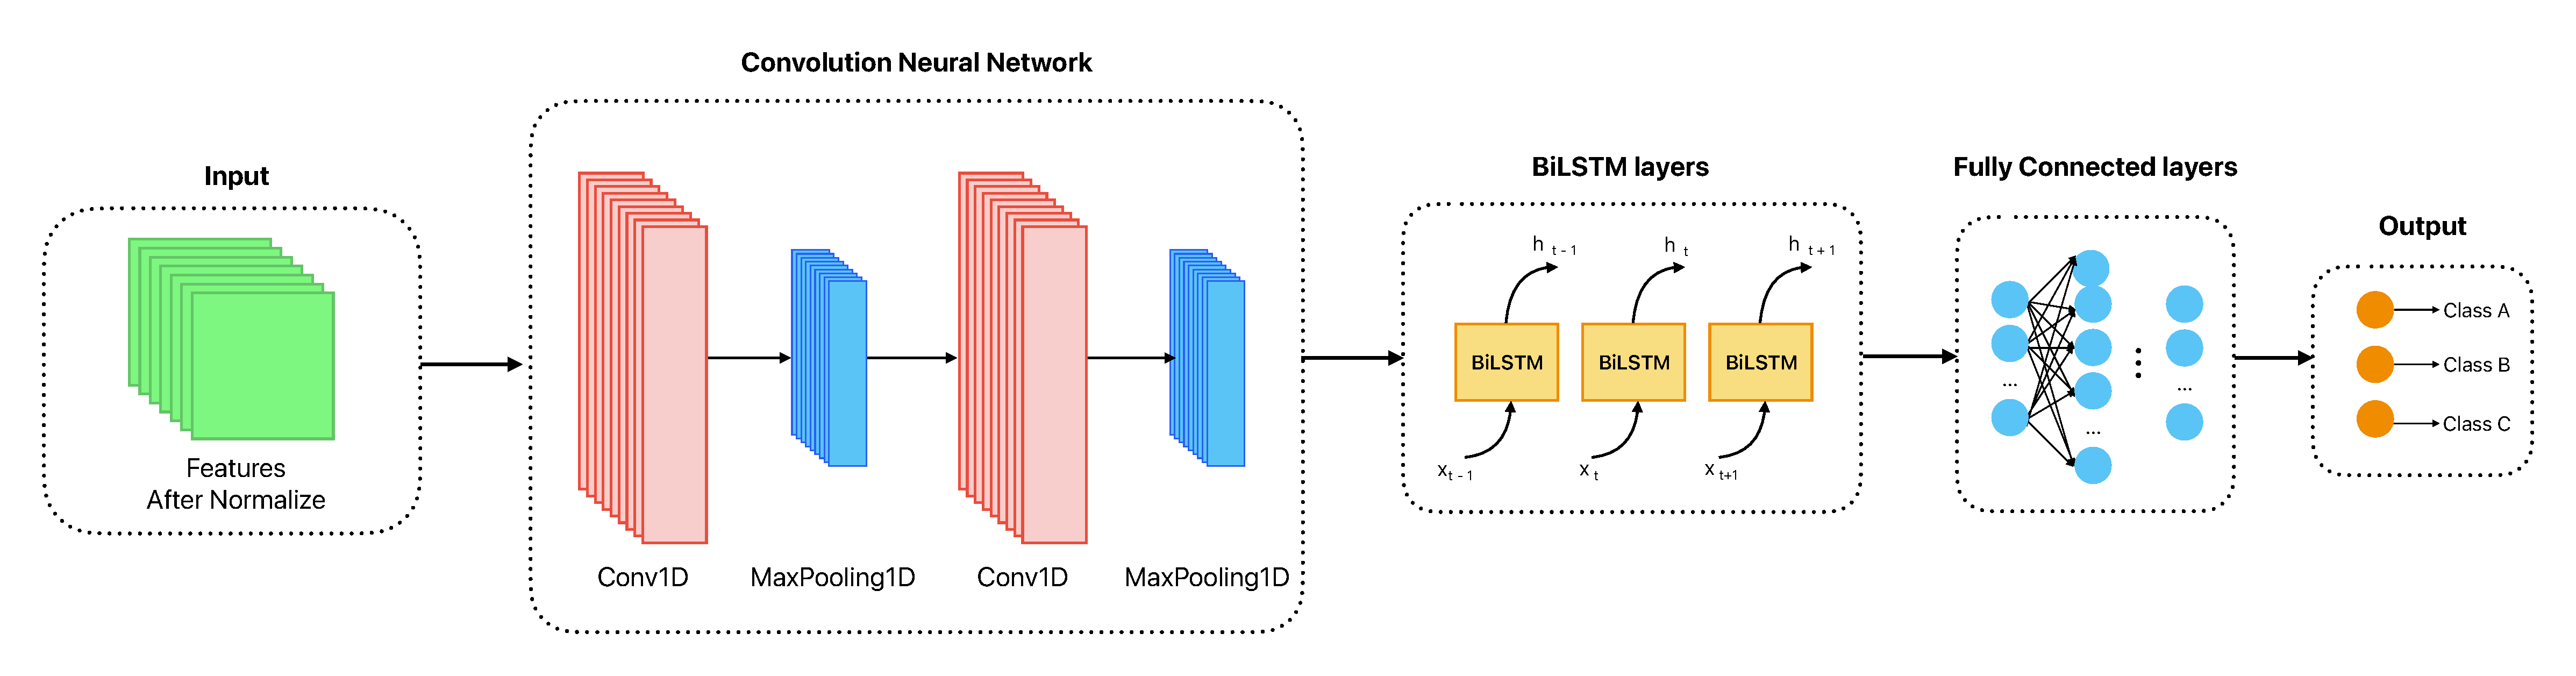
\includegraphics[width=7 in]{CNN-BiLSTM architecture.pdf}
    \caption{CNN - BiLSTM Hybrid Architecture}
    \label{fig:CNN - BiLSTM Hybrid Architecture}
\end{figure}

\begin{figure}
    \centering
    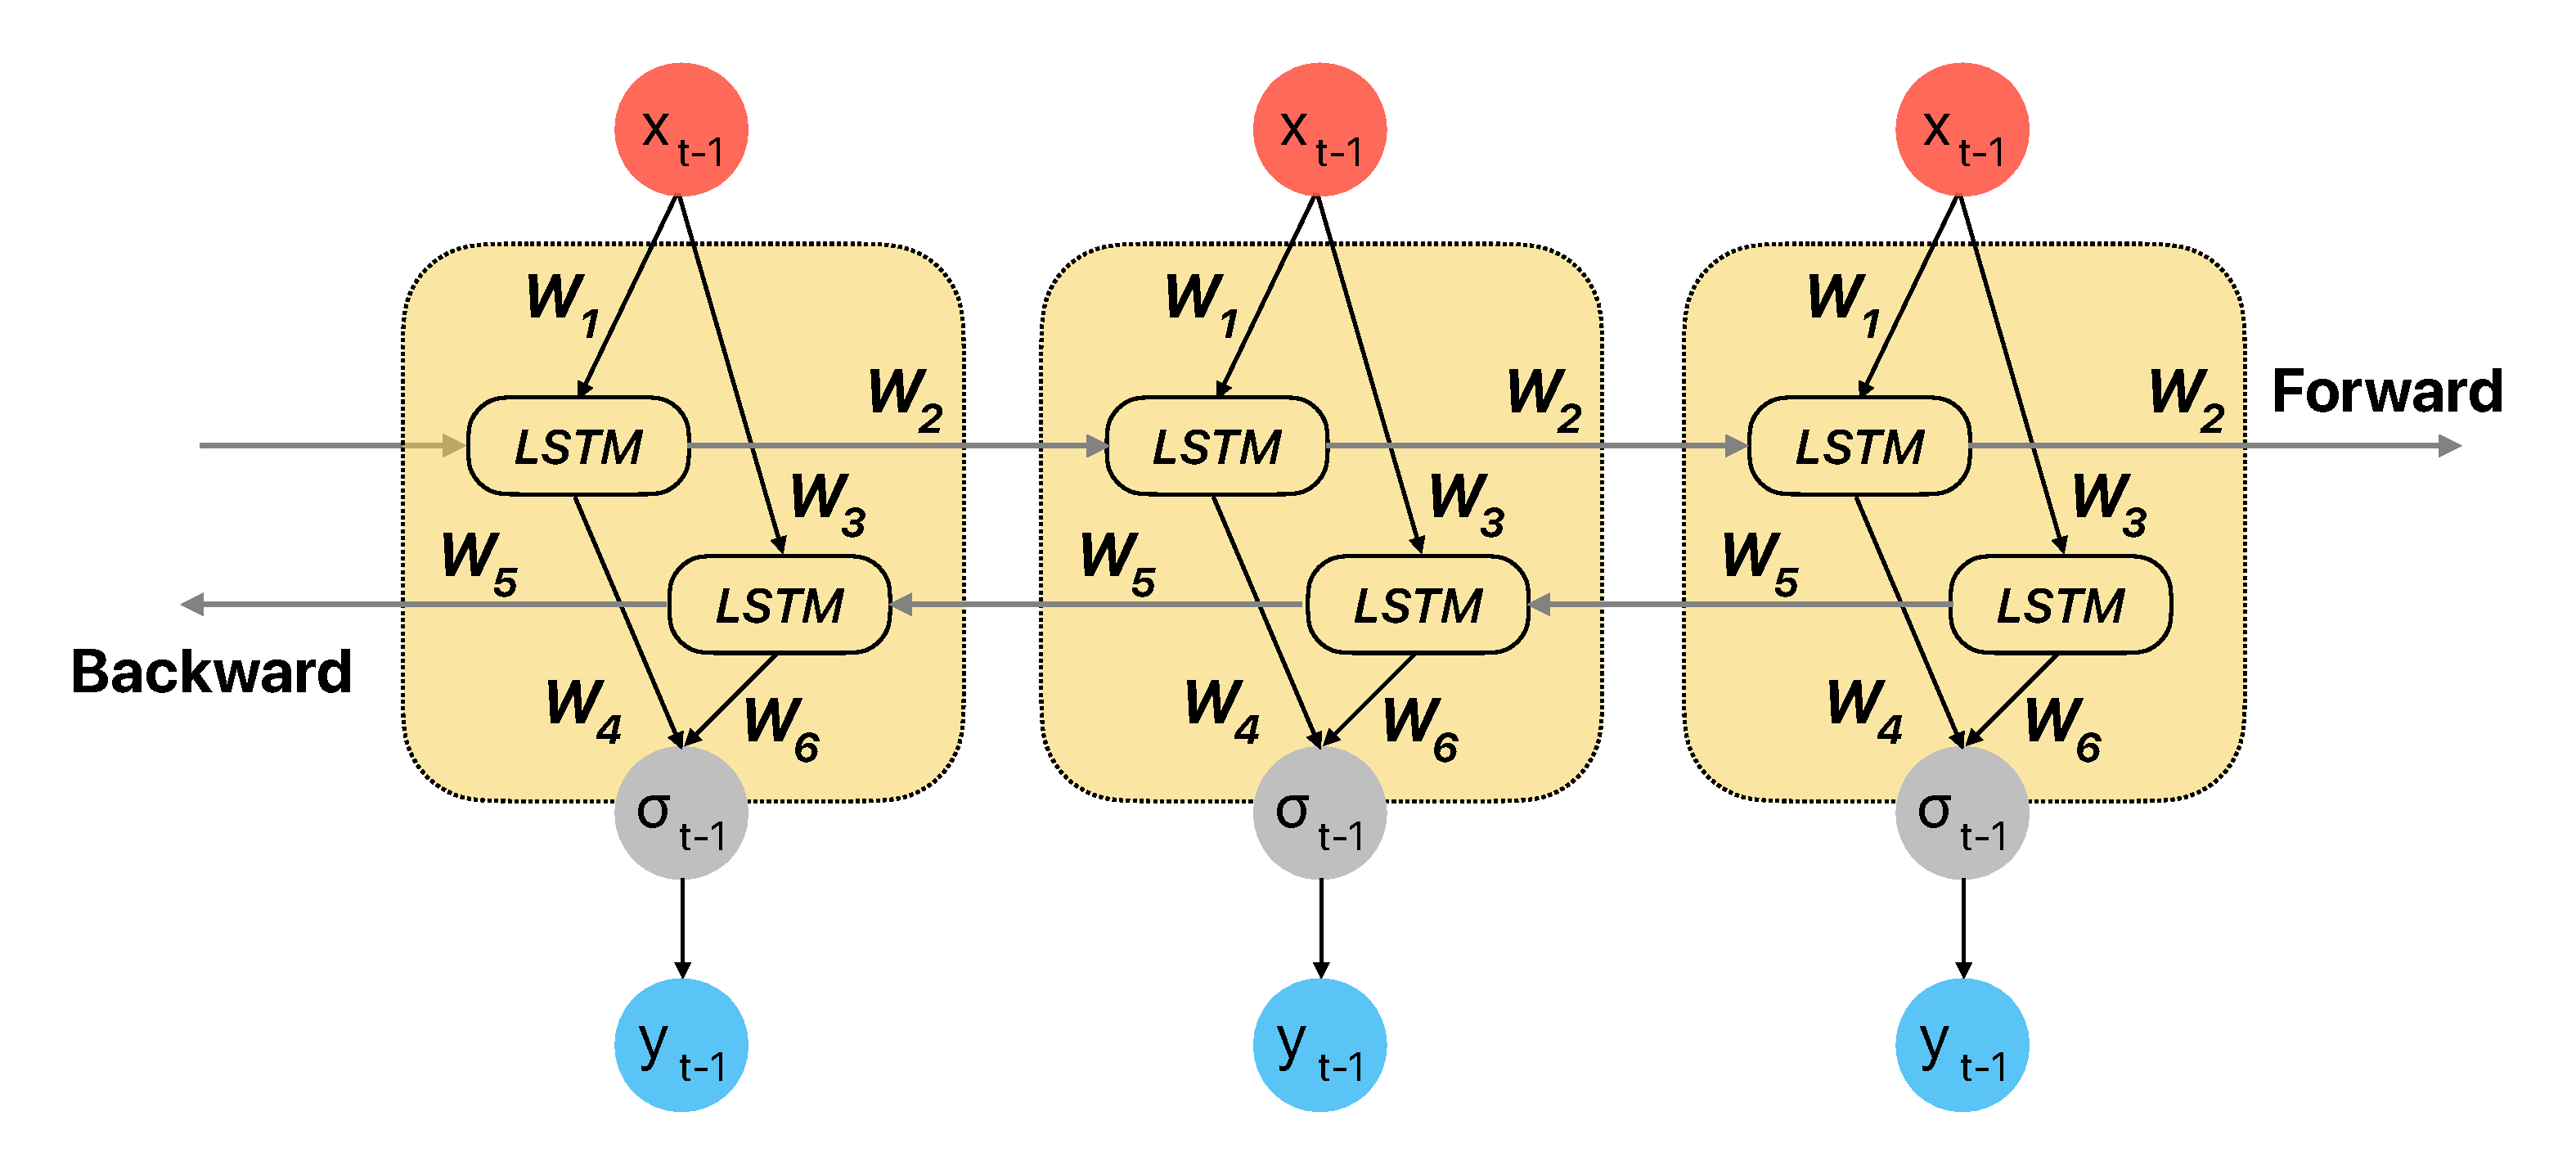
\includegraphics[width=4 in]{BiLSTM architecture.pdf}
    \caption{Bidirectional Long Short Term Memory Architecture}
    \label{fig:BiLSTM architecture}
\end{figure}

\begin{table}[]
    \centering
    \begin{tabular}{|c|c|c|}
        \hline
        \textbf{Layer} & \textbf{Nodes} & \textbf{Output Shape} \\ \hline
        \textbf{Input Layer} & & (128, 35, 54)\\
        \textbf{Conv1D} (MaxPooling1D, Dropout (0.3)) & 64 & (128, 16, 64)\\
        \textbf{Bidirectional LSTM} (Dropout (0.3), Return Sequences = True) & 256 & (128, 16, 512)\\
        \textbf{Bidirectional LSTM} (Dropout (0.3)) & 256 & (128, 512)\\
        \textbf{Dense} (Dropout (0.3), BatchNormalization) & 256 & (128, 256)\\
        \textbf{Dense} (Dropout (0.3), BatchNormalization) & 128 & (128, 128)\\
        \textbf{Dense} (Dropout (0.3), BatchNormalization) & 64 & (128, 64)\\
        \textbf{Output Layer} & 2 & (128, 2)\\
        
         \hline
    \end{tabular}
    \caption{The parameters of CNN - BiLSTM Architecture Architecture Gender Model}
    \label{tab:CNN -BiLSTM Architecture Gender}
\end{table}

\begin{table}[]
    \centering
    \begin{tabular}{|c|c|c|}
    \hline
        \textbf{Layer} & \textbf{Nodes} & \textbf{Output Shape} \\ \hline
        \textbf{Input Layer} & & (128, 35, 54)\\
        \textbf{Conv1D} (MaxPooling1D, Dropout (0.3)) & 128 & (128, 16, 128)\\
        \textbf{Conv1D} (MaxPooling1D, Dropout (0.3)) & 128 & (128, 7, 128)\\
        \textbf{Bidirectional LSTM} (Dropout (0.3), Return Sequences = True) & 256 & (128, 7, 512)\\
        \textbf{Bidirectional LSTM} (Dropout (0.3)) & 256 & (128, 512)\\
        \textbf{Dense} (Dropout (0.3), BatchNormalization) & 256 & (128, 256)\\
        \textbf{Dense} (Dropout (0.3), BatchNormalization) & 128 & (128, 128)\\
        \textbf{Dense} (Dropout (0.3), BatchNormalization) & 64 & (128, 64)\\
        \textbf{Output Layer} & 5 & (128, 5)\\
    \hline
    \end{tabular}
    \caption{The parameters of CNN -BiLSTM Architecture Architecture Age Model}
    \label{tab:CNN -BiLSTM Architecture Age}
\end{table}

\section{Experimental Result and Discussion}
\subsection{Experiment settings}

The training process is conducted on a personal computer equipped with an Intel® Core™ i7-12650H processor, and an NVIDIA GeForce RTX 3060 GPU with 8GB of RAM.
\subsection{Dataset}

In this research, we are utilizing Mozilla Voice Dataset~\cite{mozilla_voice}, containing over 350,000 recordings, which is specifically designed to study how age and gender influence the way Japanese people speak. This valuable resource is useful for researchers in various fields, including speech science, language development, and artificial intelligence. The dataset includes recordings from people of all ages, from babies to older adults. Each age group has its own unique way of speaking, which contributes to the richness and complexity of the dataset. This allows researchers to better understand the many factors that influence human communication.

\subsubsection{Dataset for Gender Recognition Model}
After The Mozilla Voice Dataset~\cite{mozilla_voice} cleansing procedures, we homogenized the dataset to solely include male and female classifications. Subsequently, we partitioned this refined dataset into subsets suitable for Gender Recognition Modeling, totaling 11,000 items. This allocation comprised 8,000 entries designated for training purposes, 2000 for validation, and 1,000  for testing. Notably, each subset maintained a balanced representation of genders, with male and female categories accounting for 50\% and 50\% of the data, respectively. It is represented in Table~\ref{tab:Distribution of samples in the Gender dataset}.

\begin{table}[htbp]
    \centering
    \begin{tabular}{|c|ccc|}
    \hline
    \textbf{Category} & \textbf{Train Dataset} & \textbf{Valid Dataset} & \textbf{Test Dataset}\\
    \hline
    Male & 4000 & 1000 & 500 \\
    Female & 4000 & 1000 & 500 \\
    \hline
    \textbf{Total} & 8000 & 2000 & 1000 \\
    \hline
    \end{tabular}
    \caption{Distribution of samples in the Gender dataset}
    \label{tab:Distribution of samples in the Gender dataset}
\end{table}

\subsubsection{Dataset for Age Recognition Model}
 Following the Mozilla Voice Dataset~\cite{mozilla_voice} refinement processes, we standardized the dataset to encompass five age categories. Subsequently, we partitioned this refined dataset into subsets tailored for age-based modeling, totaling 15,555 items. This allocation included 11,804 entries designated for training purposes, 2,951 entries for validation, and 800 entries for testing. It is noteworthy that each subset retained a balanced representation across five age classifications: teens, twenties, thirties, forties, and fifties to sixties. It is represented through Table~\ref{tab:Distribution of samples in the Age dataset}.

\begin{table}[htbp]
    \centering
    \begin{tabular}{|c|ccc|}
    \hline
    \textbf{Category} & \textbf{Train Dataset} & \textbf{Valid Dataset} & \textbf{Test Dataset}\\
    \hline
    Teens & 2361 & 590 & 160 \\
    Twenties & 2361 & 591 & 160 \\
    Thirties & 2361 & 590 & 160 \\
    Forties & 2361 & 590 & 160 \\
    Fifties - Sixties & 2360 & 590 & 160 \\
    \hline
    \textbf{Total} & 11804 & 2951 & 800\\
    \hline
    \end{tabular}
    \caption{Distribution of samples in the Age dataset}
    \label{tab:Distribution of samples in the Age dataset}
\end{table}
\subsection{Feature Extraction} 
The audio goes through a two-step process to focus on the important parts. First, it's segmented using librosa.effects.split~\cite{mcfee2015librosa}. This function identifies and separates sections with significant sounds (above an 18 dB threshold) from silent portions. You might need a separate function to reassemble these segments later. The reconstructed audio, highlighting only the non-silent parts.

In the second step, the audio is trimmed using librosa.effects.trim~\cite{mcfee2015librosa}. This function removes any silence at the beginning and end of the recording (based on a 10 dB threshold). This ensures only the relevant content remains. To analyze the impact of trimming, both the trimmed audio and its extracted harmonic component are visualized in Figure~\ref{fig:Processing Audio}.

The feature extraction process involves various sound processing techniques to capture essential characteristics from audio data. Table~\ref{tab:Feature Extraction} outlines the different sound processing techniques and the corresponding features extracted:
\begin{itemize}
    \item Delta MFCC (Mel-Frequency Cepstral Coefficients): These 13 features act like a fingerprint for a sound, capturing the way its frequency spectrum changes over time. (See in Figure~\ref{fig:MFCC extraction} and Table~\ref{tab:Feature Extraction})
    \item Delta delta MFCC: These additional 13 features add detail by describing how quickly the "fingerprint" of the sound (Delta MFCC) changes. It's like adding expression to speech through gestures. (See in Figure~\ref{fig:MFCC extraction} and Table~\ref{tab:Feature Extraction})
    \item Pitch\textbf{:} This single feature represents the sound's "highness" or "lowness," similar to the base note in music. (Search for Table~\ref{tab:Feature Extraction}, and Figure~\ref{fig:Picth-Magnitudes})
    \item Magnitude\textbf{:} This single feature reflects the overall loudness of the sound. (See in Table~\ref{tab:Feature Extraction}, and Figure~\ref{fig:Picth-Magnitudes} 
    \item Filter-Bank Energies: These 26 features provide a more intricate picture of the sound's frequency content by dividing it into sections and measuring the energy in each one. Imagine it as a detailed map compared to the fingerprint of Delta MFCC. (See in Table~\ref{tab:Feature Extraction})
\end{itemize}

The feature extraction process itself yields a total of 54 features from the audio signals (in Table~\ref{tab:Feature Extraction}). These features capture various aspects of the audio, including: Spectral content (captured by MFCCs and Filter-Bank Energies), Temporal changes (captured by Delta MFCCs and Delta-Delta MFCCs), Fundamental properties like pitch and loudness (captured by Picths and Magnitude).

These extracted features serve as a compressed representation of the original audio data, allowing machine learning models to focus on the most relevant information for tasks like gender and age recognition.
\begin{table}[htbp]
    \centering
    \begin{tabular}{|c|c|}
        \hline
        \textbf{Sound processing} & \textbf{Feature} \\
        \hline
        Delta MFCC & 13 \\
        Delta delta MFCC & 13\\
        Picth & 1 \\
        Magnitude & 1 \\ 
        Filter - Bank Energies & 26\\
        \hline
        \textbf{Total} & \textbf{54} \\
        \hline 
    \end{tabular}
    \caption{Feature Extraction}
    \label{tab:Feature Extraction}
\end{table}
\begin{figure}
    \centering
    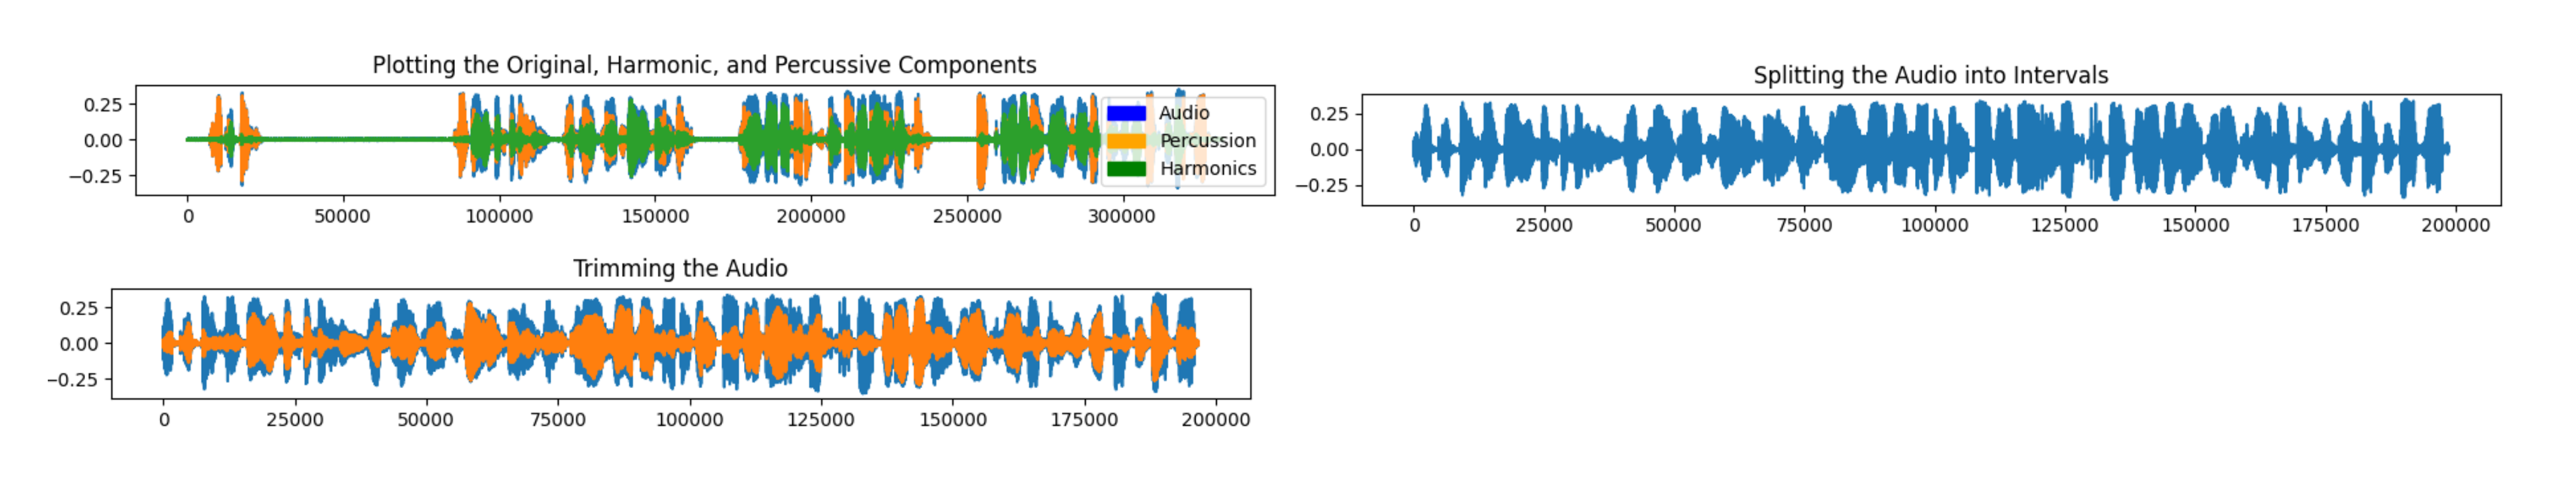
\includegraphics[width =7 in]{Processing Audio.pdf}
    \caption{Processing Audio before Extract Feature}
    \label{fig:Processing Audio}
\end{figure}
\begin{figure}
    \centering
    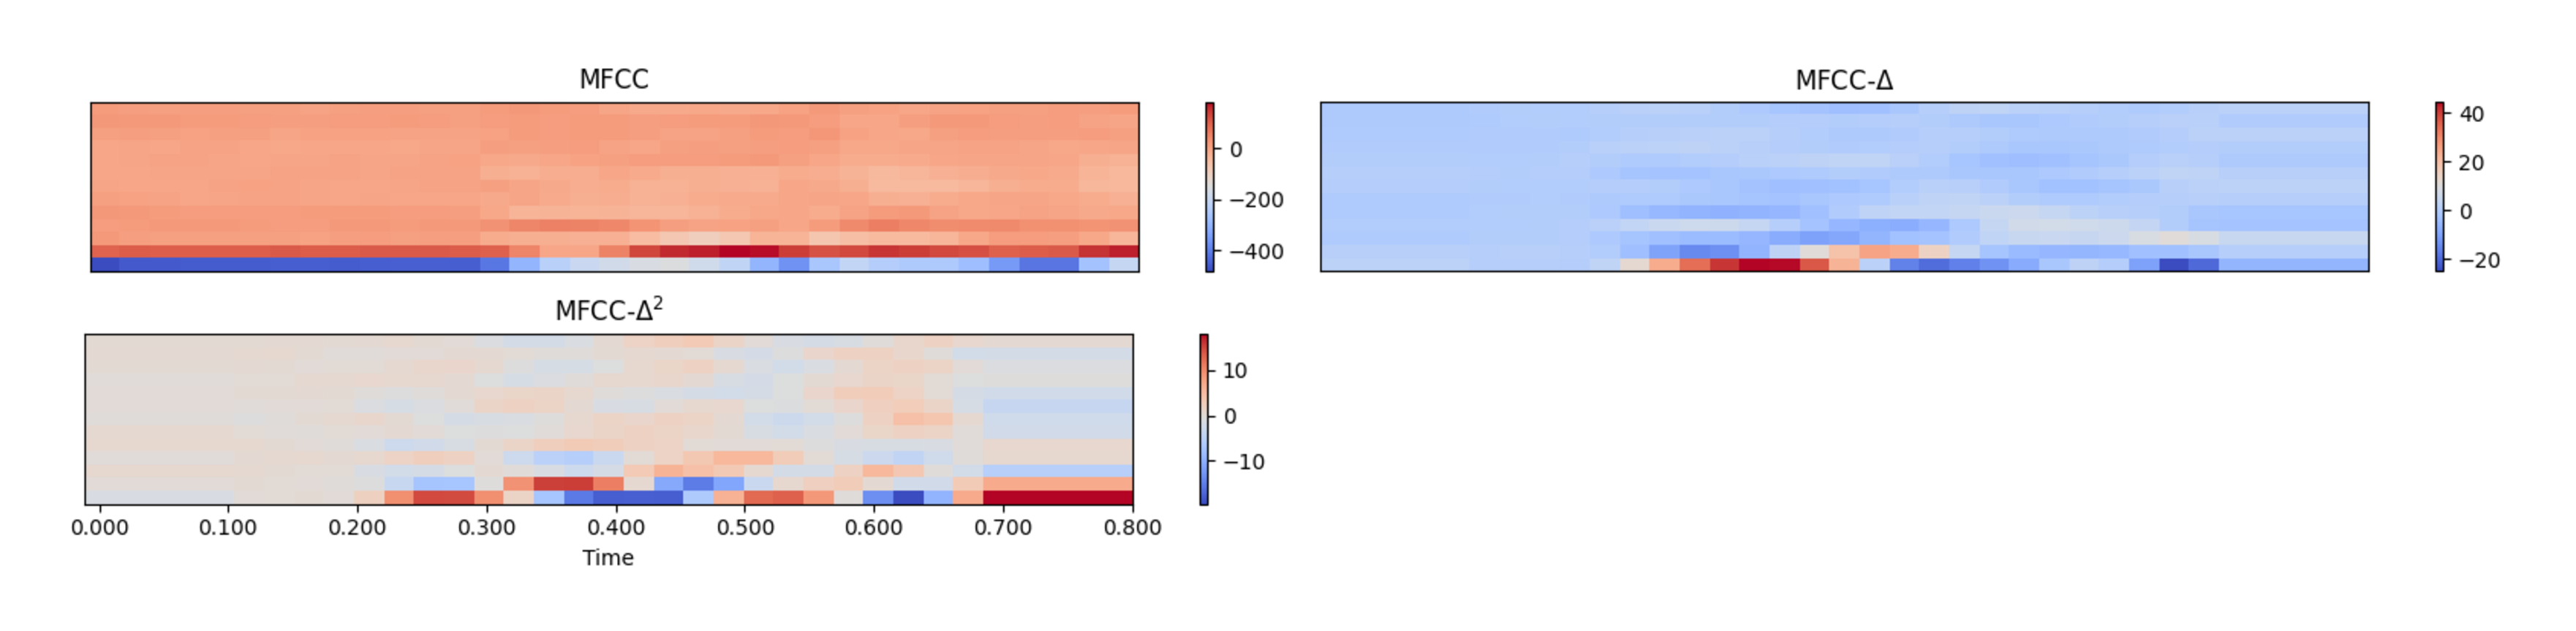
\includegraphics[width=7 in]{MFCC extraction.pdf}
    \caption{MFCC feature extraction}
    \label{fig:MFCC extraction}
\end{figure}
\begin{figure}
    \centering
    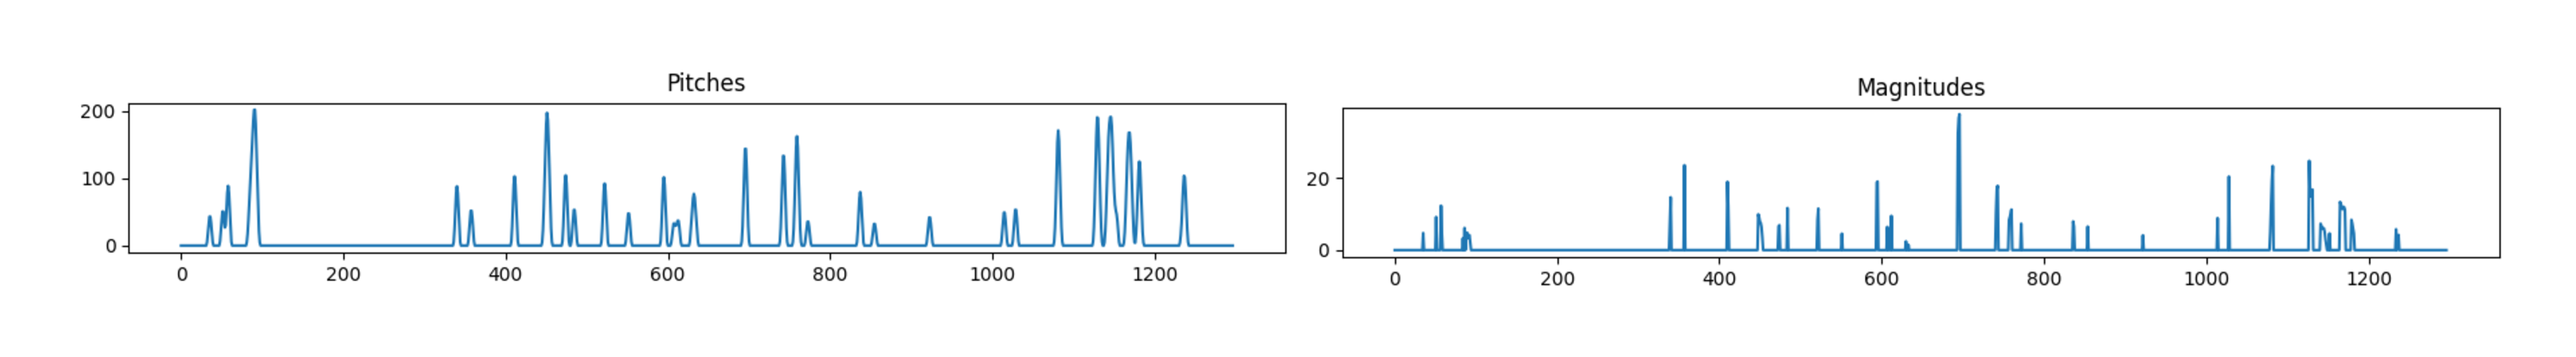
\includegraphics[width=7 in]{Pitches and Magnitudes.pdf}
    \caption{Pitches and Magnitudes}
    \label{fig:Picth-Magnitudes}
\end{figure}

\subsection{Performance Metrics}
This study employs precision, recall, and F1-score to assess the performance of our classification models.
\begin{itemize}
\item \textbf{Precision:} Precision measures the percentage of correctly identified positive instances out of all instances classified as positive by the model. It is calculated by dividing the number of true positives by the sum of true positives and false positives, as shown in Eq.~\ref{eqal: Precision}.

\begin{equation}
     \text{Precision} = \frac{\text{True Positives}}{\text{True Positives} + \text{False Positives}} 
     \label{eqal: Precision}
\end{equation}

\item \textbf{Recall:} Also known as sensitivity, recall assesses the proportion of correctly predicted positive instances among all actual positive instances in the dataset. This is computed by dividing the number of true positives by the sum of true positives and false negatives, as indicated in Eq. \ref{eqal: Recall}.

\begin{equation}
    \text{Recall} = \frac{\text{True Positives}}{\text{True Positives} + \text{False Negatives}}
    \label{eqal: Recall}
\end{equation}

\item \textbf{F1-score:} The F1-score, detailed in Eq. \ref{eqal: F1-score}, represents the harmonic mean of precision and recall. It provides a balanced evaluation by considering both precision and recall, making it particularly useful in scenarios with imbalanced datasets.

\begin{equation}
    \text{F1-score} = 2 \times \frac{\text{Precision} \times \text{Recall}}{\text{Precision} + \text{Recall}}
    \label{eqal: F1-score}
\end{equation}

\item \textbf{Macro average:} The macro average is an averaging technique used in multi-class classification tasks to calculate performance metrics like precision, recall, and F1-score across all classes, especially in imbalanced datasets. It involves computing the metric for each class individually and then averaging them, as shown in Eqs.~\ref{eqal: Macro Precision}, \ref{eqal: Macro Recall}, and \ref{eqal: Macro F1-score}.

\begin{equation}
    \text{Macro Precision} = \frac{\text{Precision of Class 1} + \text{Precision of Class 2}  + \ldots + \text{Precision of Class N}}{N}
    \label{eqal: Macro Precision}
\end{equation}

\begin{equation}
    \text{Macro F1-score} = \frac{2 \times (\text{Macro Precision} \times \text{Macro Recall})}{\text{Macro Precision} + \text{Macro Recall}}
    \label{eqal: Macro F1-score}
\end{equation}

\begin{equation}
    \text{Macro Recall} = \frac{\text{Recall of Class 1} + \text{Recall of Class 2} + \ldots + \text{Recall of Class N}}{N}
    \label{eqal: Macro Recall}
\end{equation}

\item \textbf{Weighted average:} The weighted average approach incorporates the class weights to compute precision, recall, and F1-score, reflecting the importance or contribution of each class. Weighted precision assesses the accuracy of positive predictions, weighted recall evaluates the completeness of positive predictions, and weighted F1-score provides a comprehensive model evaluation, considering class-specific significance. The formulas are provided in Eqs.~\ref{eqal: Weighted Precision}, \ref{eqil: Weighted Recall}, and \ref{eqil: Weighted F1 - Score}.

\begin{equation}
    \text{Weighted Precision} = \frac{p_1 \times w_1 + p_2 \times w_2 + \ldots + p_N \times w_N}{\text{Total Weight}}
    \label{eqal: Weighted Precision}
\end{equation}
where $p_i$ is the precision of class $i$ and $w_N$ is the weight of class $i$.

\begin{equation}
    \text{Weighted Recall} = \frac{r_1 \times w_1 + r_2 \times w_2 + \ldots + r_N \times w_N}{\text{Total Weight}}
    \label{eqil: Weighted Recall}
\end{equation}
where $r_N$ is the recall of class $i$ and $w_N$ is the weight of class $i$.

\begin{equation}
    \text{Weighted F1 - Score} = \frac{f_1 \times w_1 + f_2 \times w_2 + \ldots + f_N \times w_N}{\text{Total Weight}}
    \label{eqil: Weighted F1 - Score}
\end{equation}
where $f_N$ is the F1-Score of class $i$ and $w_N$ is the weight of class $i$.

\end{itemize}

\subsection{Experimental Result of Models' Architecture}

For all three architectures, Long Short-Term Memory (LSTM), Hybrid Convolutional Neural Networks with Bidirectional (CNN BiLSTM), and RezoNet, utilized in the age and gender recognition model, the training process remains consistent. We normalize the features, resulting in 54 features. During training, we employ the Adam optimizer with a learning rate set to 0.0001, use categorical cross-entropy as the loss function, and assess model performance using categorical cross-entropy as the evaluation metric. Additionally, we incorporate early stopping with a patience parameter set to 5 to prevent overfitting, enabling the restoration of the best weights. This uniform training approach ensures a fair comparison of the performance of all three architectures.

\subsubsection{Long - Short Term Memory (LSTMs) architecture}

The LSTM architecture for gender recognition achieved an accuracy of 93.50\%, indicating its proficiency in classifying male and female voices. Precision, recall, and F1-score for the male class were 0.96178, 0.90600, and 0.93306, respectively, while for the female class, they were 0.91115, 0.96400, and 0.93683, respectively (see Table~\ref{tab:Experience of Gender Recognize Model with LSTM Architecture}). These metrics reflect a balanced performance, with macro and weighted averages for precision, recall, and F1-score around 0.936 and 0.935, respectively.

In the age recognition task using the same LSTM architecture, the model achieved an accuracy of 64.25\%. Precision, recall, and F1-score varied across age groups, with the Forties age group exhibiting the highest precision of 0.75887 and the Thirties age group showing the highest recall of 0.74375. Overall, the model demonstrated a moderate performance, with macro and weighted averages for precision, recall, and F1-score around 0.656 and 0.642, respectively (see Table~\ref{tab:Experience of Age Recognize Model with LSTMs Architecture}).

Comparing the two tasks, the gender recognition model exhibited higher accuracy and performance metrics compared to the age recognition model. This suggests that the LSTM architecture is more effective in distinguishing between male and female voices compared to classifying age groups. Further research and model refinement may be necessary to improve the performance of age recognition models using LSTM architecture.
\begin{table}[htbp]
    \centering
    \begin{tabular}{|c|cccc|}
        \hline
        \textbf{Class} & \textbf{Precision} & \textbf{Recall} & \textbf{F1-score} & \textbf{Support} \\
        \hline
        Male & 0.96178 & 0.90600 & 0.93306 & 500 \\
        Female & 0.91115 & 0.96400 & 0.93683 & 500 \\
        \hline
        \textbf{Accuracy} & \multicolumn{2}{c}{} & 0.93500 & 1000 \\
        \textbf{Macro Average} & 0.93647 & 0.93500 & 0.93495 & 1000 \\
        \textbf{Weighted Average} & 0.93647 & 0.93500 & 0.93495 & 1000 \\
        \hline
    \end{tabular}
    \caption{Experience of Gender Recognize Model with LSTMs Architecture}
    \label{tab:Experience of Gender Recognize Model with LSTM Architecture}
\end{table}

\begin{table}[htbp]
    \centering
    \begin{tabular}{|c|cccc|}
        \hline
        \textbf{Class} & \textbf{Precision} & \textbf{Recall} & \textbf{F1-score} & \textbf{Support} \\
        \hline
        Teens & 0.67227 & 0.64375 & 0.66883 & 160 \\
        Twenties & 0.49763 & 0.65625 & 0.56604 & 160 \\
        Thirties & 0.65746 & 0.74375 & 0.69795 & 160 \\
        Forties & 0.75887 & 0.66875 & 0.71096 & 160 \\
        Fifties - Sixties& 0.69595 & 0.64375 & 0.66883 & 160 \\
        \hline
        \textbf{Accuracy} &  && 0.64250 & 800 \\
        \textbf{Macro Average} & 0.65643 & 0.64250 & 0.64345 & 800 \\
        \textbf{Weighted Average} & 0.65643 & 0.64250 & 0.64345  & 800 \\
        \hline
    \end{tabular}
    \caption{Experience of Age Recognize Model with LSTMs Architecture}
    \label{tab:Experience of Age Recognize Model with LSTMs Architecture}
\end{table}
\subsubsection{RezoNet Architecture}
The RezoNet architecture for gender recognition achieved an accuracy of 83.10\%. For the male class, precision, recall, and F1-score were 0.96884, 0.68400, and 0.80188, respectively. For the female class, these metrics were 0.75580, 0.97800, and 0.85266, respectively. The macro and weighted averages for precision, recall, and F1-score were approximately 0.862 and 0.831, indicating a well-balanced performance across both classes (see Table~\ref{tab:Experience of Gender Recognize Model with RezoNet Architecture}).

In the age recognition task using the RezoNet architecture, the model achieved an accuracy of 44.88\%. Precision, recall, and F1-score varied across age groups, with the Teens group exhibiting the highest precision of 0.52475 and the Thirties group showing the highest recall of 0.71875. Overall, the model demonstrated a moderate performance, with macro and weighted averages for precision, recall, and F1-score around 0.467 and 0.448, respectively (see Table~\ref{tab:Experience of Age Recognize Model with RezoNet Architecture}).

These results highlight the effectiveness of the RezoNet architecture in gender recognition, achieving high accuracy and balanced performance, while also demonstrating its potential for age classification, although with a slightly lower accuracy and performance compared to gender recognition.
\begin{table}[htbp]
    \centering
    \begin{tabular}{|c|cccc|}
        \hline
        \textbf{Class} & \textbf{Precision} & \textbf{Recall} & \textbf{F1-score} & \textbf{Support} \\
        \hline
        Male & 0.96884 & 0.68400 & 0.80188 & 500 \\
        Female & 0.75580 & 0.97800 & 0.85266 & 500 \\
        \hline
        \textbf{Accuracy} & \multicolumn{2}{c}{} & 0.83100 & 1000 \\
        \textbf{Macro Average} & 0.86232 & 0.83100 & 0.82727 & 1000 \\
        \textbf{Weighted Average} &0.86232 & 0.83100 & 0.82727  & 1000 \\
        \hline
    \end{tabular}
    \caption{Experience of Gender Recognize Model with RezoNet Architecture}
    \label{tab:Experience of Gender Recognize Model with RezoNet Architecture}
\end{table}

\begin{table}[htbp]
    \centering
    \begin{tabular}{|c|cccc|}
        \hline
        \textbf{Class} & \textbf{Precision} & \textbf{Recall} & \textbf{F1-score} & \textbf{Support} \\
        \hline
        Teens & 0.52475 & 0.33125 & 0.40613 & 160 \\
        Twenties & 0.32919 & 0.33125 & 0.33022 & 160 \\
        Thirties & 0.41071 & 0.71875 & 0.52273 & 160 \\
        Forties & 0.48148 & 0.40625 & 0.44068 & 160 \\
        Fifties - Sixties& 0.59350 & 0.45625 & 0.51590 & 160 \\
        \hline
        \textbf{Accuracy} &  &  & 0.44875 & 800 \\
        \textbf{Macro Average} & 0.46793 & 0.44875 & 0.44313 & 800 \\
        \textbf{Weighted Average} & 0.46793 & 0.44875 & 0.44313  & 800 \\
        \hline
    \end{tabular}
    \caption{Experience of Age Recognize Model with RezoNet Architecture}
    \label{tab:Experience of Age Recognize Model with RezoNet Architecture}
\end{table}

\subsubsection{Hybrid of Convolutional Neural Networks and Bidirectional Long Short-Term Memory Architecture (CNN - BiLSTM)}
The CNN - BiLSTM hybrid architecture for gender recognition achieved an accuracy of 93.10\%. Precision, recall, and F1-score for the male class were 0.93535, 0.92600, and 0.93065, respectively. For the female class, these metrics were 0.92673, 0.93600, and 0.93134, respectively. The macro and weighted averages for precision, recall, and F1-score were approximately 0.931, indicating a well-balanced performance across both classes (see Table~\ref{tab:Experience of Gender Recognize Model with CNN - BiLSTM Hybrid Architecture}).

In the age recognition task using the CNN - BiLSTM hybrid architecture, the model achieved an accuracy of 69.75\%. Precision, recall, and F1-score varied across age groups, with the Thirties group exhibiting the highest precision of 0.79054 and the Twenties group showing the highest recall of 0.73125. Overall, the model demonstrated a moderate performance, with macro and weighted averages for precision, recall, and F1-score around 0.701 and 0.697, respectively (see Table~\ref{tab:Experience of Age Recognize Model with CNN - BiLSTM Hybrid Architecture}).

These results underscore the effectiveness of the CNN - BiLSTM hybrid architecture in gender recognition, achieving high accuracy and balanced performance, while also showing promising results for age classification, although with slightly lower accuracy and performance compared to gender recognition.
\begin{table}[htbp]
    \centering
    \begin{tabular}{|c|cccc|}
        \hline
        \textbf{Class} & \textbf{Precision} & \textbf{Recall} & \textbf{F1-score} & \textbf{Support} \\
        \hline
        Male & 0.93535 & 0.92600 & 0.93065 & 500 \\
        Female & 0.92673 & 0.93600 & 0.93134 & 500 \\
        \hline
        \textbf{Accuracy} & \multicolumn{2}{c}{} & 0.93100 & 1000 \\
        \textbf{Macro Average} & 0.93104 & 0.93100 & 0.93100 & 1000 \\
        \textbf{Weighted Average} & 0.93104 & 0.93100 & 0.93100 & 1000 \\
        \hline
    \end{tabular}
    \caption{Experience of Gender Recognize Model with CNN - BiLSTM Hybrid Architecture}
    \label{tab:Experience of Gender Recognize Model with CNN - BiLSTM Hybrid Architecture}
\end{table}

\begin{table}[htbp]
    \centering
    \begin{tabular}{|c|cccc|}
        \hline
        \textbf{Class} & \textbf{Precision} & \textbf{Recall} & \textbf{F1-score} & \textbf{Support} \\
        \hline
        Teens & 0.63871 & 0.61875 & 0.62857 & 160 \\
        Twenties & 0.59281 & 0.61875 & 0.60550 & 160 \\
        Thirties &  0.79054 & 0.73125 & 0.75974 & 160 \\
        Forties &   0.70213 & 0.82500 & 0.75862 & 160 \\
        Fifties - Sixties & 0.70213 & 0.82500 & 0.75862 & 160 \\
        \hline
        \textbf{Accuracy} &  &  & 0.69750 & 800 \\
        \textbf{Macro Average} & 0.70118 & 0.69750 & 0.69751 & 800 \\
        \textbf{Weighted Average} & 0.70118 & 0.69750 & 0.69751 & 800 \\
        \hline
    \end{tabular}
    \caption{Experience of Age Recognize Model with CNN - BiLSTM Hybrid Architecture}
    \label{tab:Experience of Age Recognize Model with CNN - BiLSTM Hybrid Architecture}
\end{table}



\subsection{Comparison Architecture}

This section compares three different architectures: Long Short-Term Memory (LSTM), a Hybrid Convolutional Neural Networks with Bidirectional (CNN - BiLSTM) architecture, and RezoNet with a Gender and Age Model. We will analyze their strengths and weaknesses to determine the most suitable approach for our task.

\begin{table}[]
    \centering
    \begin{tabular}{|c|c|c|c|c|c|c|} \hline 
        \textbf{Types} &  \multicolumn{3}{|c|}{\textbf{Gender Recognize Model}}&  \multicolumn{3}{|c|}{\textbf{Age Recognize Model}}\\ \hline
        \textbf{Performance Matrix} & \textbf{LSTM} & \textbf{RezoNet} & \textbf{CNN-BiLSTM} & \textbf{LSTM}& \textbf{RezoNet} & \textbf{CNN-BiLSTM}\\ \hline 
        \textbf{Accuracy} & 0.93500& 0.83100 & 0.93100& 0.64250& 0.44875& 0.69750\\
        \textbf{Macro Precision}& 0.93647& 0.86232& 0.93104& 0.65643& 0.46793& 0.70118\\
        \textbf{Macro Recall}& 0.93500& 0.83100& 0.93100& 0.64250& 0.44875& 0.69750\\
        \textbf{Macro F1-score}& 0.93495& 0.82727& 0.93100& 0.64345& 0.44313& 0.69751\\ \hline
    \end{tabular}
    \caption{Experimental result of all Architectures}
    \label{tab:Experimental result of all Architectures}
\end{table}
\subsubsection{Gender Recognize Model}

The analysis of the gender prediction models over epochs reveals that the LSTM model consistently outperforms the others in terms of both accuracy, loss overtime (in Figure~\ref{fig:Gender_valid}), and the experiment results table~\ref{tab:Experimental result of all Architectures}. Initially, the LSTM starts with a lower accuracy compared to the CNNs-BiLSTM but quickly surpasses it around the third epoch, reaching and maintaining the highest accuracy of approximately 0.92 from the eighth epoch onward. Its loss also steadily decreases, stabilizing at around 0.2 by the fourteenth epoch. The CNNs-BiLSTM model, while initially strong and achieving a high accuracy quickly, shows a more gradual improvement and stabilizes with a slightly lower peak accuracy of about 0.91 and a final loss of around 0.25. In contrast, the RezoNet model exhibits significant volatility in both accuracy and loss, showing large fluctuations throughout the training period and ending with an accuracy of about 0.88 and a loss of around 0.22. Overall, the LSTM model demonstrates the most robust and stable performance, making it the best choice among the three for gender prediction based on these metrics.

\begin{figure}
    \centering
    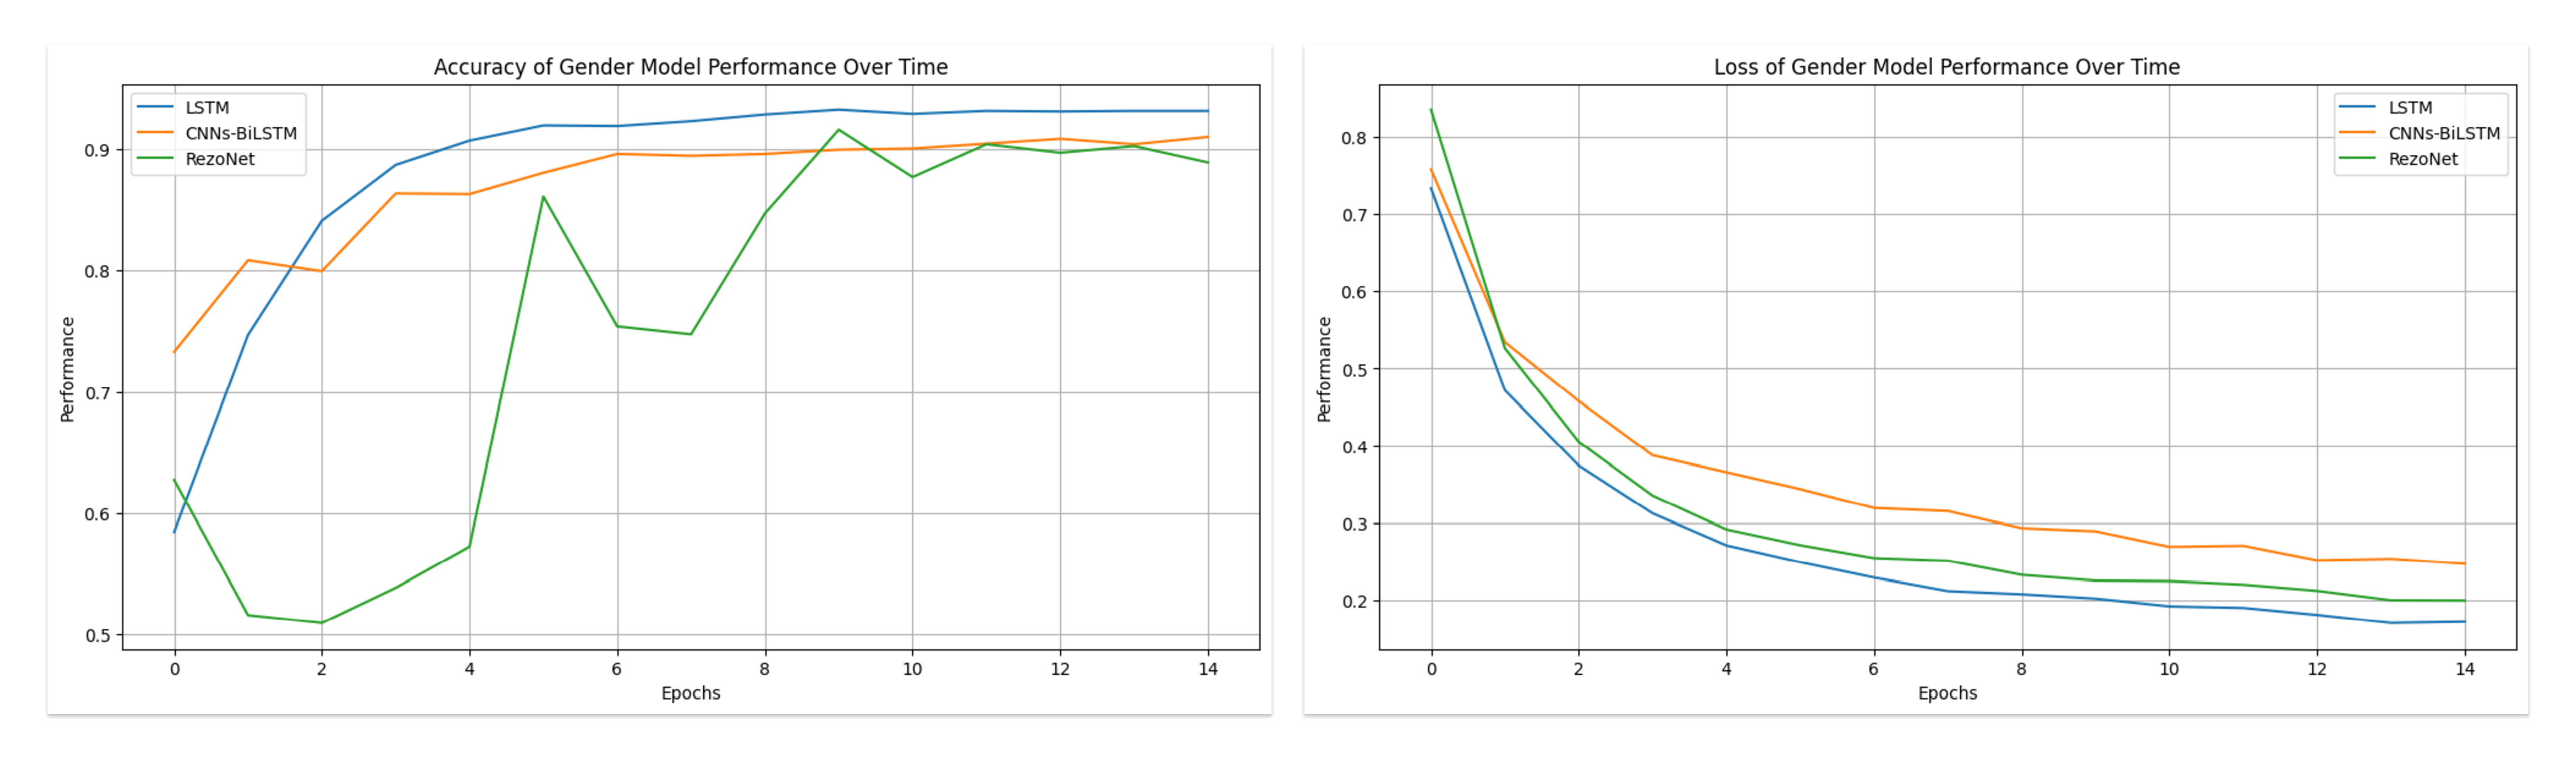
\includegraphics[width=7 in]{Gender Model.pdf}
    \caption{Accuracy and Loss of Gender Model Performance Over Time}
    \label{fig:Gender_valid}
\end{figure}

\subsubsection{Age Recognize Model}
The provided images depict the performance of three models (LSTM, CNNs-BiLSTM, and RezoNet) for age recognition over time, with the  table summarizing the experiment results (in table~\ref{tab:Experimental result of all Architectures}), images showing accuracy and loss (in Figure~\ref{fig:Age_valid}). The CNNs-BiLSTM model exhibits the best performance, starting with a strong initial improvement and consistently improving over the epochs, surpassing both LSTM and RezoNet around epoch 30 and reaching the highest accuracy (about 0.65) by the end of the training period. In contrast, the LSTM model shows gradual improvement, starting better than RezoNet but remaining consistently lower than CNNs-BiLSTM, ultimately achieving moderate accuracy (around 0.5). The RezoNet model, however, has the lowest accuracy performance, showing slow and steady improvement and ending with around 0.35 accuracy. In terms of loss, CNNs-BiLSTM also demonstrates the most significant reduction, starting with relatively high loss but quickly decreasing to about 0.6 by the end of the training period. The LSTM model shows a steady decrease in loss, starting higher than CNNs-BiLSTM but lower than RezoNet, ending at around 1.0. RezoNet has the highest initial loss and the slowest reduction, remaining higher than both CNNs-BiLSTM and LSTM throughout the epochs and ending at about 1.4. In summary, CNNs-BiLSTM outperforms both LSTM and RezoNet in terms of both accuracy and loss, achieving the best performance for age recognition, while LSTM shows moderate performance, and RezoNet is the least effective with the lowest accuracy and highest loss.

\begin{figure}
    \centering
    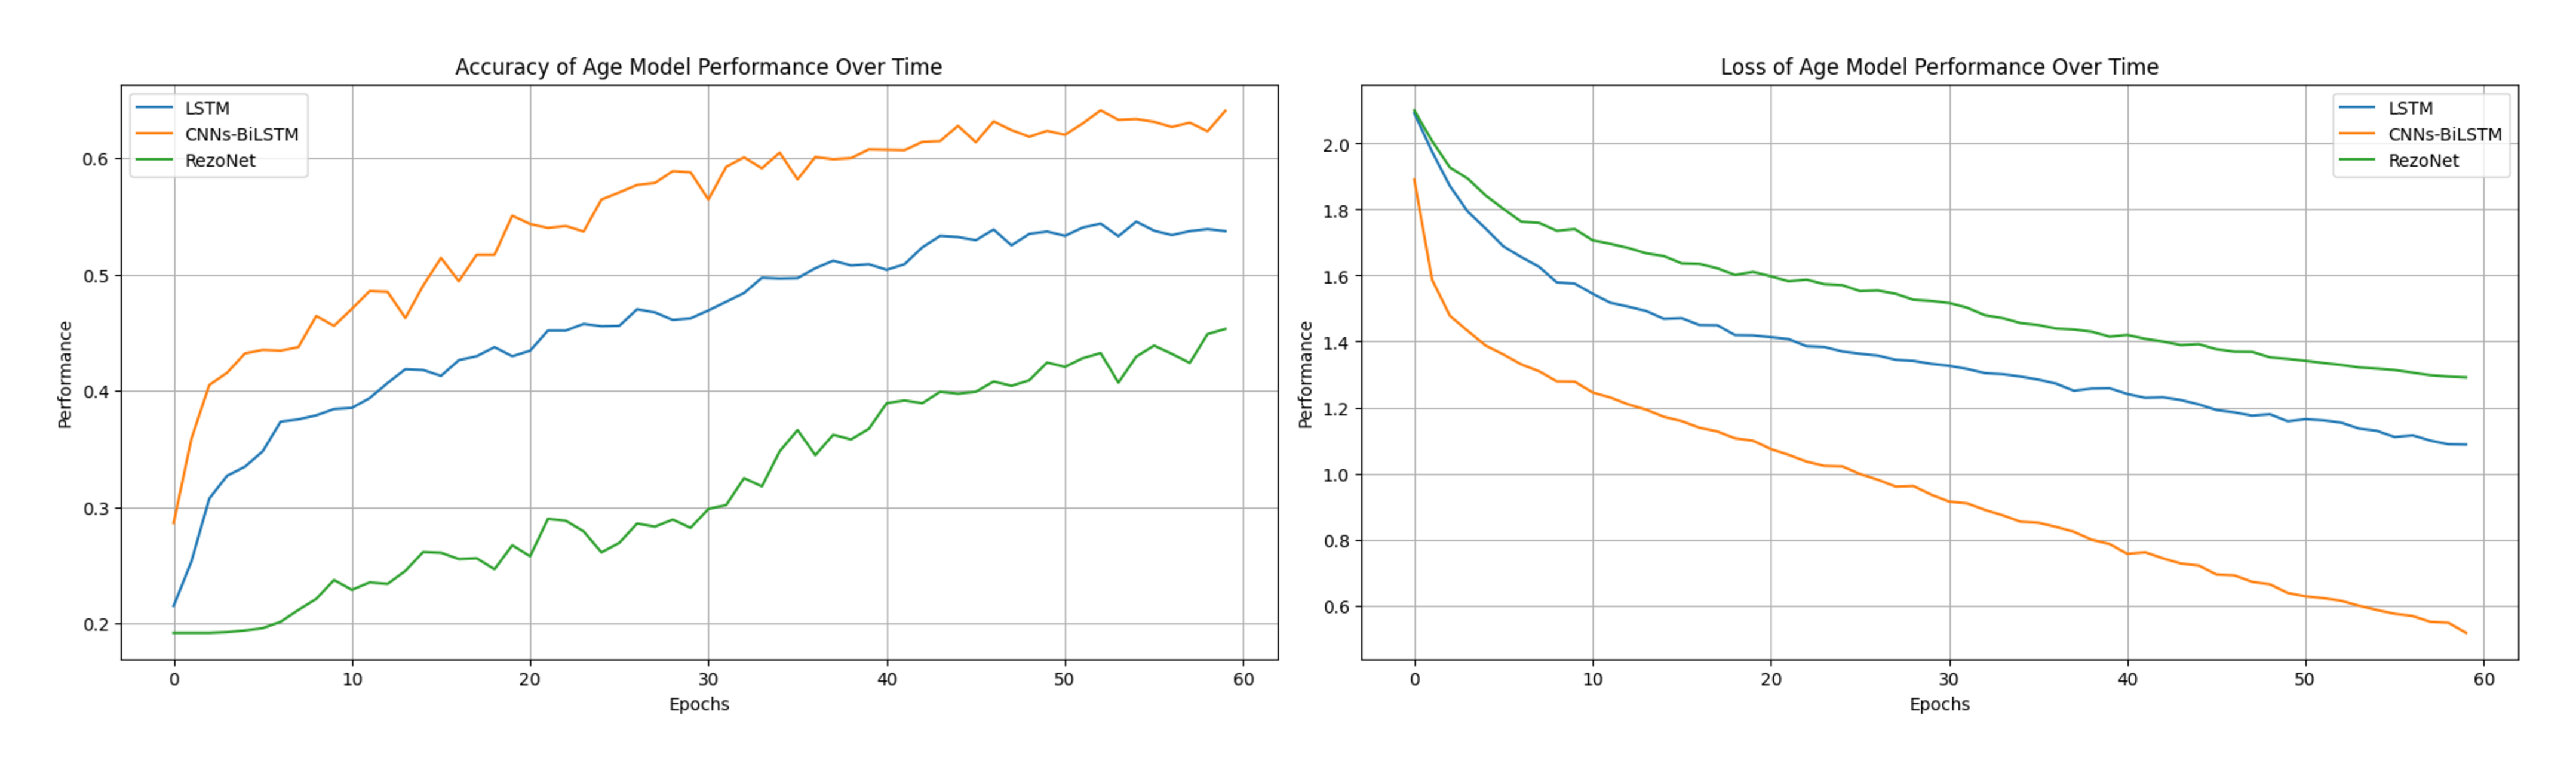
\includegraphics[width=7 in]{Age Model.pdf}
    \caption{Accuracy and Loss of Age Model Performance Over Time}
    \label{fig:Age_valid}
\end{figure}
\subsection{Discussion about Performance of Architecture}

After conducting extensive training and testing processes, our findings revealed that Long Short-Term Memory (LSTM) and Hybrid Convolutional Neural Networks with Bidirectional (CNN-BiLSTM) architectures demonstrated superior accuracy (in Table~\ref{tab:Experimental result of all Architectures}), faster training, and quicker processing times in voice-based age and gender recognition tasks compared to RezoNet. This superiority is attributed to their proficiency in capturing temporal dependencies through LSTM layers and extracting relevant temporal features directly from audio signals via Conv1D layers, instead of Conv2D layers in RezoNet. Additionally, the parameter efficiency of Conv1D layers alleviates computational burdens during both training and inference, facilitating accelerated processing. The hierarchical feature learning capabilities of CNN-BiLSTM architectures, amalgamating CNNs' hierarchical feature extraction with LSTMs' long-range dependency capture, enable better representation of complex patterns in voice data. Furthermore, the parallelization potential of LSTM and CNN-BiLSTM architectures during training further expedites the process, particularly on parallel processing hardware like GPUs and TPUs. Overall, the heightened model complexity and adaptability of LSTM and CNN-BiLSTM architectures significantly contribute to their superior performance in voice-based age and gender recognition tasks compared to RezoNet.

\section{Conclusion and Future Enhance}
This study compared three deep learning architectures: Long-Short Term Memory (LSTM), RezoNet Architecture and Hybrid Convolutional Neural Network - Bidirectional Long Short-Term Memory (CNNs-BiLSTM) for Voice-based Age and Gender Recognition. Among the three architectures, CNNs-BiLSTM emerged as the most effective, achieving the highest accuracy for age recognition. It also delivered a competitive performance in gender recognition, surpassing both LSTM and RezoNet.

While the CNNs-BiLSTM architecture showed promise, the study also identified exciting avenues for future research. These include using larger and more diverse datasets that encompass various ethnicities and languages to improve the model's generalizability. Additionally, exploring a multi-task learning approach that tackles age and gender recognition simultaneously could lead to further performance gains. Finally, incorporating Explainable AI techniques would provide valuable insights into the factors influencing the model's decisions, leading to more transparent and trustworthy systems.

\section{Acknowledgement}
\bibliographystyle{IEEEtran}  % IEEE
\bibliography{Mybib}          % IEEE

\end{document}


